\documentclass[twoside]{styles/uocthesis}

\usepackage{subcaption}
\captionsetup{compatibility=false}


\usepackage[pdftex]{graphicx} %Loading the package
\graphicspath{{figures/}} %Setting the 


\usepackage[acronym]{glossaries}
\usepackage{booktabs}
\usepackage{styles/gnuplot-lua-tikz}
\usepackage{tikz}
\usepackage{amsmath}
\usepackage{enumitem}




\Title{Interactive Machine Learning for annotation and  of Object Detection and Segmentation}
\Author{Oliver Batchelor}
\Year{2018}

\Supervisor{Prof. Richard Green}
\Department{Department of Computer Science}

\makeglossaries




\begin{document}

\prelimpages


\titlepage


\abstract{%

Applying deep learning to new domains usually implies a data collection and annotation problem. While several large datasets exist and provide a great deal of utility, there is a need to apply deep learning to new domains more easily, and to more easily experiment without the burden of spending a large amount of time upfront to annotate data. This thesis explores some the ideas and tools needed for rapid prototyping with image data and convolutional neural networks. 
Specifically I have focused on image segmentation and object detection methods where I've developed ``Human in the loop'' annotation methods based on the idea that validating annotations is faster than manually inputting those validations from scratch.


}

\tableofcontents



\printglossaries

\newacronym{FCN}{FCN}{Fully Convolutional Network}
\newacronym{FPN}{FPN}{Feature Pyramid Network}


\newacronym{FP}{FP}{False Positive}
\newacronym{FN}{FN}{False Negative}

\newacronym{TN}{TN}{True Negative}
\newacronym{TP}{TP}{True Positive}


\newacronym{IOU}{IOU}{Intersection Over Union}
\newacronym{VOC}{VOC}{Visual Object Classes}
\newacronym{mIOU}{mIOU}{mean Intersection Over Union}

\newacronym{CRF}{CRF}{Conditional Random Field}

\newacronym{RELU}{ReLU}{Rectified Linear Unit}
\newacronym{PRELU}{PReLU}{Parameterised Rectified Linear Unit}
\newacronym{DECAF}{DeCAF}{Deep Convolutional Activation Feature}

\newacronym{FPN}{FPN}{Feature Pyramid Network}


\newacronym{NLL}{NLL}{Negative Loss Likelihood}
\newacronym{BCE}{BCE}{Binary Cross Entropy}
 
\newacronym{COCO}{CoCo}{Microsoft Common Objects in Context}
\newacronym{ILSVRC}{ILSVRC}{ImageNet Large Scale Visual Recognition Challenge}

\newacronym{CNN}{CNN}{Convolutional Neural Network}
\newacronym{MCDNN}{MCDNN}{Multi-Column Deep Neural Network}

\newacronym{SIFT}{SIFT}{Scale Invariant Feature Transform}
\newacronym{SURF}{SURF}{Speeded Up Robust Features}

\newacronym{ALOI}{ALOI}{Amsterdam Library of Images}
\newacronym{MSR}{MSR}{Microsoft Research}
\newacronym{AMT}{AMT}{Amazon Mechanical Turk}

\newacronym{BOW}{BoW}{Bag of Words}
\newacronym{BOVW}{BoVW}{Bag of Visual Words}

\newacronym{ANN}{ANN}{Approximate Nearest Neighbour}
\newacronym{SGD}{SGD}{Stochastic Gradient Descent}
\newacronym{ASGD}{ASGD}{Asynchronous Stochastic Gradient Descent}
\newacronym{LOO}{LOO}{Leave One Out}

\newacronym{NCA}{NCA}{Neighbourhood Components Analysis}
\newacronym{MEGM}{MEGM}{Mean square Error's Gradient Minimisation}

\newacronym{KNN}{kNN}{k-Nearest Neighbour}

\newacronym{MSE}{MSE}{Mean Squared Error}
\newacronym{LMNN}{LMNN}{Large Margin Nearest Neighbour}
\newacronym{NCM}{NCM}{Nearest Class Mean}

\newacronym{SVM}{SVM}{Support Vector Machine}

\newacronym{PCA}{PCA}{Principle Components Analysis}
\newacronym{DRLIM}{DrLIM}{Dimensionality Reduction by Learning an Invariant Mapping}
\newacronym{SGDR}{SGDR}{Stochastic Gradient Descent with Restarts}
 
\newacronym{GPU}{GPU}{Graphics Processing Unit} 
\newacronym{CPU}{CPU}{Central Processing Unit}




\acknowledgments{%
I will like to thank all the hedgehogs, without there help this
thesis would not be a reality.}

\textpages




\chapter{Introduction}

In this chapter I discuss firstly the broader context of research which relates to interactive annotation as it applies to this work. I discuss the topics in general, but also focus on applications to image processing with \gls{CNN}s. In section \ref{sec:closest} I then spend some time to compare and contrast the most specific research efforts most similar to this work.

\section{Research goals and contributions}

The central thesis to this dissertation is that annotation of data can be performed as a collaboration between human and machine learning algorithm. This by itself is not new idea, and is known as 'human in the loop' machine learning. Given the wide variety of visual recognition task, and thus different kinds of work-flow for annotation - I look to provide the best set of tools to empower the human annotator.

Specifically I look at two aspects where a machine learning algorithm assists a human annotator. The first and main focus is verification based annotation where a human annotator annotates a dataset by validating machine generated predictions.

The second focus is organising data and example selection - allowing an annotator to sort images, then find the best images to annotate first and then find mistakes or inconsistencies. 

A large part of crowd sourced annotation is having cross verification. I look at how a machine learning algorithm can help verify a dataset instead, to weed out errors by finding and showing inconsistencies in the provided data.

I explore the topic in a modern scenario using \gls{CNN}s, and aim to show the approach is very practical for annotation of a range of visual recognition datasets. I do this through developing tools for human in the loop image annotation and performing a series of experiments to answer questions and validate my ideas. I also demonstrate it's use on a series of real world image annotation tasks.


\subsection {Thesis summary and contributions}

This thesis is split into roughly two parts, firstly works which stand alone - and is presented first, chapter \ref{chap:focus} where I look at the effect of cropping and resolution on image classification, and \ref{chap:metric} where I experiment with a new method of metric learning for instance recognition, a kind of n-way siamese network. 

The rest of the thesis from \ref{chap:bootstrap} onward is devoted to the central topic of the thesis, namely human in the loop machine learning. In chapter \ref{chap:bootstrap} I discuss verification based annotation for segmentation data where images are annotated by drawing masks over areas of interest. I explore several angles for assisted image annotation, and conclude that the verification based bootstrapping process to be the most promising. Contrary to popular belief that \gls{CNN}s require much data and much training time. I demonstrate the opposite that using few images, and also very little training time a \gls{CNN} can be trained to a level to provide very real assistance to a human annotator. 

In chapters \ref{chap:object_detection} I experiment with a state of the art object detection \gls{CNN} model and look at properties useful for human in the loop annotation. I look at practical aspects of training, including training one class at a time, cyclical learning rates and experiment on several small scale (but real world) datasets. 


Chapter \ref{chap:object_detection} is devoted to the design and implementation of a human in the loop annotation system 

I also look at example selection methods, where I look at how an annotation tool can facilitate annotation workflows for different kinds of image data. I briefly explore methods of effectively reviewing existing annotations for consistency, and how unlabelled data can be more effectively sorted and processed.

I demonstrate the utility of the tool by annotating several new object detection datasets (and validate it on a few older ones),  and collaborate with others who use it to annotate datasets.



\subsection {Rapid prototyping}

Not only is it necessary to collect and annotate data - one of the primary questions asked when considering the use of machine learning is 'How many examples are necessary?'. To which the usual answer is to by experimental validation where part of the data is held back and used to test the effectiveness of training on the other part. In this work I don't change 



\section {Thesis structure}


\section {Background}

Crowd sourcing. Human in the loop. verification based annotation.

Uncertainty, active learning.

Related ideas are are those which aim to make more effective use of data available. This includes methods to enrich existing data such as semi-supervised learning and hard example mining \cite{Jin2018, Yu2018, Canevet2014}, as well as those aiming to accelerate the learning process by sampling the data in the right order, including curriculum learning and self paced learning.

Transfer learning attempts to accelerate learning on a new domain by using knowledge gained through learning on another (usually much larger and more general) domain. It has been shown that (especially for images with \gls{CNN}s) that models trained on these datasets can be re--purposed in a variety of useful ways.


\subsection {Crowd Sourcing}

The most common approach to annotating a dataset is crowd sourcing. Crowd sourcing enlists the services of many in order to provide 

Most large scale datasets are created with some form of crowd sourcing, notable examples ImageNet classification \cite{JiaDeng2009}, Coco object detection \cite{Lin2014} or Cityscapes street scenes \cite{Cordts2016} are all created with crowd sourcing. 

In order to get a lot of people to contribute there exist methods such as gamification, where the task is turned into a fun game  e.g. a game Quick Draw \cite{Ha2017}, or presenting the task as proof of humanness \cite{Goodfellow2013a}. Citizen science uses volunteers to perform tasks, for example to count penguins, identify species or identify planets \cite{Simpson2014, Masters2016}. Often the feeling of contributing to something meaningful, or the novelty of having your name as a contributor is enough to bring people to be involved.

If there exists no easy way to bring people to help for free, then use of labour markets such as \gls{AMT} are an option. These markets enable an employer to pay for mechanical tasks involving human intelligence. Many large scale datasets such as ImageNet \cite{Russakovsky2015} are built with \gls{AMT}. 


\subsection{Human in the loop}

Human in the loop machine learning encompasses a range of machine learning techniques which utilise human input in effective ways. Either by providing assistance to a human annotator with verification based annotation, or by having the annotator assist a learner which tries to make the most out of annotator time, such as active learning.

Machine learning datasets often contain a lot of so called ``easy'' examples. These examples often dominate both the annotation process where human time is spent needlessly annotating similar easy examples, and in the learning process where the learning algorithm spends much of it's computation time on examples which are already handled well. 


\subsection{Verification based annotation}

\begin{figure}[h]
  \centering
  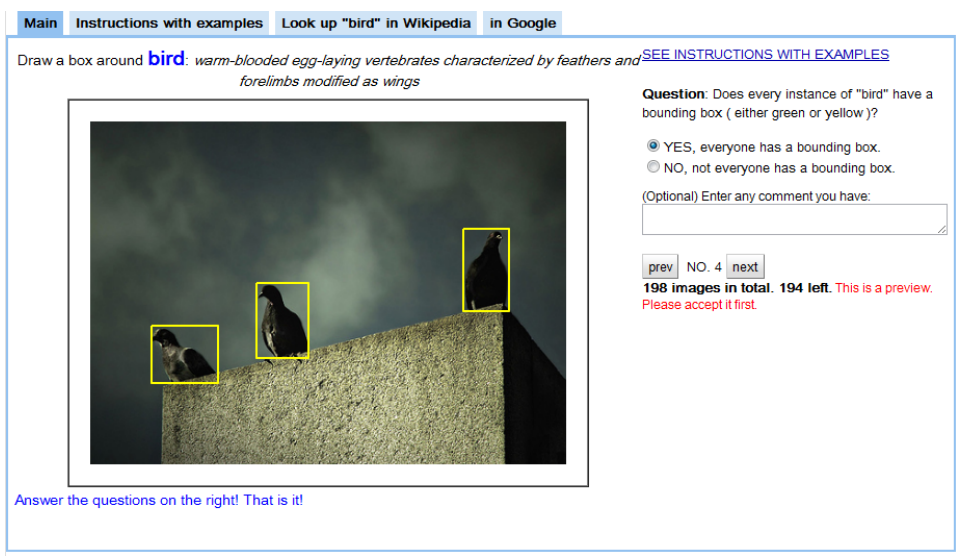
\includegraphics[width=0.9\linewidth]{introduction/crowdsourcing_annotation.jpg}
  \caption{Crowd sourcing image verification task in \cite{Su2012a}}  
  \label{fig:captcha}
\end{figure}

I coin the term verification based annotation, where machine annotations are checked and verified by a human annotator. Although the idea has played a central role in many previous works, it is not given an easily recognisable term to distinguish it for example from other kinds of Human in the Loop machine learning such as Active Learning (and is often put in the same basket). A selection of verification based methods, many of them discussed in detail below \cite{Yao2012, McNeill2011, Adhikaria2018, Castrejon2017, Papadopoulos2016, Russakovsky2015a}. 

Verification also plays a large part in ensuring consistency even between human annotators in crowd sourcing efforts, where the annotations of any one user cannot be fully trusted - users are tasked with cross verifying each others' annotations in many of these efforts, an example of a crowd sourcing task for annotating boxes on Image-net \cite{Su2012a}.

Weaker algorithms (machine learning or otherwise) can be used to generate proposals which can be then validated by an annotator. An example of this is in \cite{McNeill2011} where computer vision algorithms generate proposed counts of a penguin colony, and a human operator marks false negatives and false positives.

Human verification is fast, in \cite{Papadopoulos2016} reports a yes/no verification as taking 1.6 seconds on average. For a full annotation of an \gls{ILSVRC} image \cite {Su2012a} the time to draw a bounding box is reported at 26 seconds (42 seconds after quality control), but \cite{Papadopoulos2017} reports only 7 seconds per box using a more effective input method involving clicking extremities of objects rather than selecting corners. 

\begin{figure}[h]
  \centering
  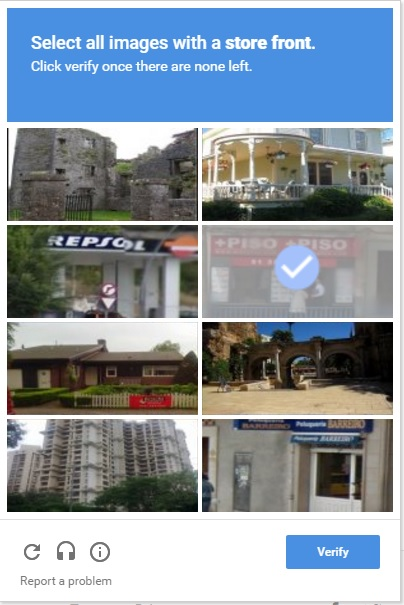
\includegraphics[width=0.9\linewidth]{introduction/recaptcha.jpeg}
  \caption{reCAPTCHA dialog showing multi-image verification task}  
  \label{fig:captcha}
\end{figure}

The human ability to verify many examples at once has often be used, for example in recent tasks presented by the well known reCAPTCHA \cite{von2008recaptcha} a grid of images is presented asking a user to select all instances containing a particular object or type of scene, this is shown in figure \ref{fig:captcha}. To my knowledge there is no study confirming if visually validating multiple occurrences together is more efficient than validating single occurrences, but given it's wide use it seems that is likely the case. 

Previous studies on verification based annotation such as \cite{Papadopoulos2016} focuses on localisation for the ImageNet dataset which features typically few large object instances per image (due to it's origins as an image classification dataset), with smaller instances often in the background. On domains with many smaller objects such as in biological studies of animals, verifying many instances at once should be much more effective. 


\subsection{Example selection and active Learning}

One prominent ``human in the loop'' method is active learning. Active learning revolves around picking the best set of examples for a human to annotate making most effective use of their time. Picking the best examples is often based around an uncertainty measure, where examples which a model is most uncertain about would often be the hard cases which are most useful for learning. 
 
While a \gls{CNN} used for classification provides some measure of uncertainty in it's output by way of it's softmax outputs, but this is usually not recommended and deemed unreliable. In \cite{Guo2017} it is shown that modern neural network architectures often systematically over estimate confidence, 

\gls{CNN}s with accurate uncertainty measures are much in their infancy, especially for more complex tasks such as object detection. However recent research gone into more effectively quantifying uncertainty in \gls{CNN}s with tools such as Bayesian \gls{CNN}s \cite{Gal2017} and other methods of estimating uncertainty have arisen such as ensemble variation \cite{Beluch2018} or minibatch variation \cite{Chang2017}. 

Specific to object detection one recent approach is to measure the stability of predicted boxes when noise is added to inputs \cite{Kao2018}. Another idea is to measure consistency between bounding box proposals \cite{Kao2018, Brust2018, Le2018}. Current state of the art object detectors such as \gls{SSD} \cite{Liu2016a}, or \gls{RCNN} \cite{Wang2011a} produce a multitude of box proposals - as such the variation can be measured.

Another measure used in active learning is expected change. An example of this is \cite{Vondrick2011} for video annotation, in which frames are selected for annotation which cause large expected change in the object track. Another example is \cite{Xu2017} where the expected change in an image's segmentation is used for the purpose of selecting which superpixels. 

Another related but distinct idea is making the best use of the examples available and in the best order. Curriculum learning and self paced learning \cite{Kumar2010} are research efforts devoted to this goal. Curriculum learning aims to learn from the most informative examples of a dataset in order to learn faster and more reliably, (a recent example is \cite{Katharopoulos2018}) self paced learning also attempts to have the learning algorithm also determine which examples are hard and easy as it progresses.


\subsection{Semi-supervised learning}

Semi-supervised methods are another active research area which aims to make use of more minimal labelling - either incomplete labelling or weak labelling. An example is in upgrading datasets with only category labels to datasets with localisation, one method involves using the internal activity of a \gls{CNN} to infer location of objects in an image \cite{Sivic2015}.

Semi-supervised ideas like hard example mining \cite{Loshchilov, } is commonplace in object detection. Negative examples are not explicitly annotated but found when false positives occur during training.

Properties such as temporal consistency can also be used to infer labels which are not explicitly annotated, if an annotated object exists on one frame in a video then it probably exists in adjacent frames, too.


\subsection{Interactive machine learning}

Many human in the loop processes (those which use human refinement to train a learner) are technically a form of interactive machine learning, but more specifically interactive machine learning uses human inputs to make predictions or modify it's behaviour directly.

Interactive machine learning is often used for segmentation where it takes considerable effort to input a segmentation mask, much more than to draw a bounding box for example. Object selection for example the GrabCut algorithm \cite{Rother} can be used to find object masks with approximate user input, such as scribbles or bounding box selection. Such a tool can be used iteratively to create, then refine an annotation with the annotator observing the output and making changes to the inputs.  LabelMe \cite{Russell2007} interface provides a scribble based object mask creation tool in this mould. 

More recently, the same ideas have been applied using \gls{CNN}s where a model can be trained to predict an object mask based on simulated user input, for example clicks \cite{Xu2016b, Boroujerdi2017}, bounding boxes \cite {Xu2017} or extreme points \cite{Maninis2017}. Human input can also be used to refine an output for example in medical segmentation \cite{Wang2017}, or for image colourisation \cite{Zhang} where it's primary purpose is to provide a more intuitive editing tool.

A contrasting interactive approach is to have a model provide outputs designed to be easily editable, such as PolygonRNN \cite{Castrejon2017} which provides automatic object selection by bounding box, but provides outputs as a polygon rather than as a mask. The benefit of this approach is that a polygon can be edited more precisely and fed back into training directly.




\subsection {Transfer learning}

Transfer learning is the idea of taking knowledge gained from a base task, and applying it to another. The most prominent and widespread use of transfer learning is perhaps the use of fine tuning or feature extraction.  Where models trained on classification tasks (typically ImageNet \cite{JiaDeng2009}) are re-purposed for usually much smaller scale tasks in different ways. 

\gls{DECAF} \cite{Donahue2014} showed features extracted from the hidden layers of a \gls{CNN} were directly transferable to achieve the then state of the art on a number of image tasks, including classification and as a much stronger replacement for the hand crafted \gls{SURF} descriptor \cite{bay2006surf}.  Specifically they used AlexNet  \cite{Krizhevsky2012} trained on ImageNet \cite{JiaDeng2009}.

In \cite{Yosinski} it is shown that the transfer-ability of features depends on the distance between the base task to the target task, and that using a pre--trained network can even improve generalisation after fine tuning (as compared to training from scratch).

Fine tuning retrains a network for a new task, typically using a lower (or zero) learning rate for some parts in order to preserve the learned 

The use of pre-trained models is now commonplace in adapting \gls{CNN} to new domains, with repositories of state of the art models pre-trained on large datasets existing for most machine learning frameworks (for example the PyTorch \cite{Paszke2017} model zoo. 

It is becoming standard practice, models for other tasks - for example segmentation or object detection are usually based around a network (the so called backbone of a network) which has previously been trained on a classification task. Examples include the widely used \gls{FPN} network, \cite{Lin2017a} where a base network, for example a ResNet \cite{He} or a DenseNet \cite{Huang2016} backbone which operates from high resolution to low, is combined by a secondary path which operates from low resolution to high with shortcut connections between, combining a pattern seen before in the segmentation U--Net \cite{Ronneberger2015} architecture with pre-trained models.

The \gls{FPN} is now used as a base model in a variety of state of the art segmentation and object detection methods, and seems widely applicable to a variety of tasks by attaching different network ``heads'' specific to the task at hand (such as classification, regression etc.).




\section {Most similar projects to this work}
\label{sec:closest}

\subsection {Interactive Object Detection \cite{Yao2012}}
Interactive object detection \cite{Yao2012} describes a human in the loop interactive annotation system, where an incremental object detector (Hough forest) is trained as a user corrects annotations provided by the system. 

The user interface consists of the ability to delete incorrectly predicted instances (\gls{FP}) and to add new bounding boxes where the object detector failed to produce them (\gls{FN}). A user study was done and found that \gls{FN} were almost twice as expensive as \gls{FP} to correct. Though it is not mentioned the exact mechanism required from the user to implement these edits. It could be because the cost of drawing a box is faster than selecting one for deletion.


The work in this thesis has a similar focus in many aspects, notably using an object detection algorithm with a predict--refine--train loop. 

In contrast, an emphasis is placed on active learning and predicting the amount of time required for a user to correct the object predictions provided by the model, in this thesis the focus on enabling the user. 

Hough forests \cite{Gall2011} are used as an online learning method for the purposes of being fast to train and fast for inference. One disadvantage of hough forests is that when annotation mistakes are made then the decision trees which arise from those mistakes can not be reversed. 

In this thesis I focus on using \gls{CNN} based object detectors (particularly RetinaNet \cite{Lin2017} and \gls{FPN} \cite{Lin2017a}) for the same purpose, which benefit from recent developments in object detection and are in general much more capable object detectors. Compared to the hough forests described, training can be slower, but inference is much faster on a modern \gls{GPU} than the figures provided for the hough forest (13 seconds).



\subsection{Fluid Annotation \cite{Andriluka2018}}
\begin{figure}[h]
  \centering
  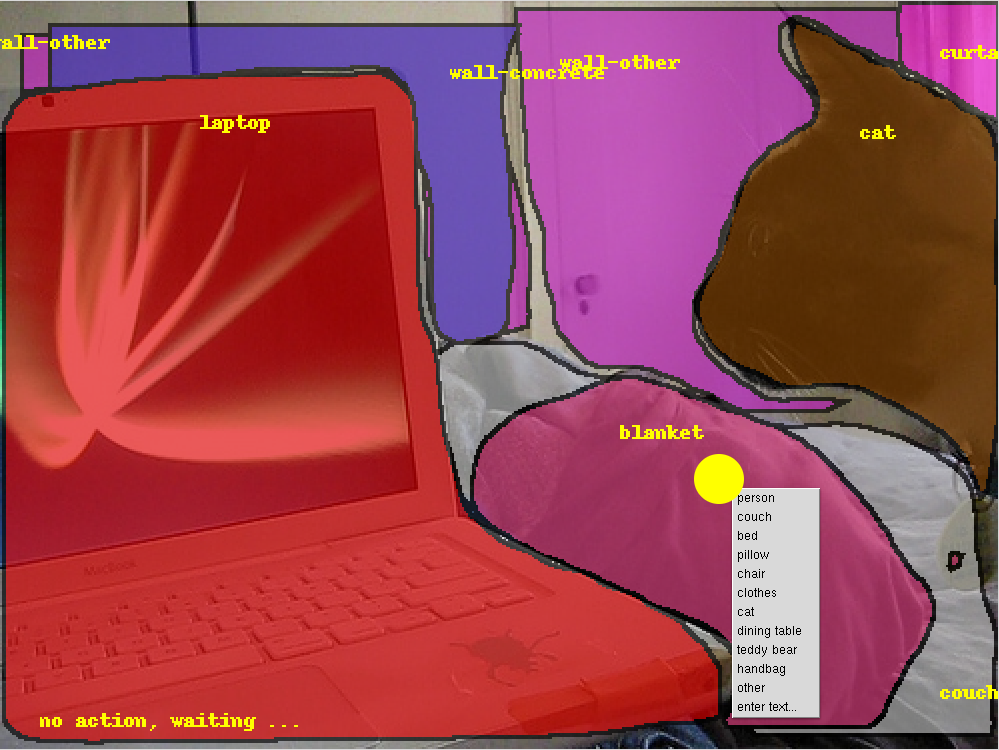
\includegraphics[width=0.9\linewidth]{introduction/fluid_annotation.png}
  \caption{User interface for Fluid Annotation \cite{Andriluka2018}}  
  \label{fig:fluid_annotation}
\end{figure}

Fluid annotation is an interactive human in the loop approach for instance segmentation. They point out three key points of their approach, the use of a strong neural network model, editing an entire image at once (as opposed to asking questions about each annotation one by one), and the approach to empower the annotator rather than employing clever methods to select examples (such as active learning). An example of the user interface is shown in figure \ref{fig:fluid_annotation}.

A key difference to my approaches is that I focus on annotating and experimentation with new domains, using transfer learning as a tool to enable online learning of the new domain. The strong neural network provides a power annotation aid, but limits you to annotate images in the same domain as that network (which is fine for many tasks).

\subsection{Faster Bounding Box Annotation for Object Detection in Indoor Scenes}
In \cite{Adhikaria2018}, an object detection dataset is annotated in two parts, first a small split is annotated and used to train an initial model, then the remaining data is annotated by having the human annotator validate and refine model predictions. My approach is similar in many ways, the difference is that I focus on iterating annotation and training immediately with an online learning approach.

\subsection {PolygonRNN}
Polygon-RNN \cite{Castrejon2017} uses a predict, refine, train approach in generating segmentation masks (as polygons), where a model is trained to segment generic objects then it can be fine tuned for a specific tasks where a user first provides a bounding box around an object, the model predicts a polygon and the refines the polygon and it is fed back for training.

\subsection {We Don't Need No Bounding Boxes}
In \cite{Papadopoulos2016}, a classification dataset is enriched with bounding box information. Instead of annotating a dataset from scratch - a model, and dataset are iteratively refined together by asking questions of a human annotator. They initially bootstrap a model using semi-supervised methods with per--image labels. A simple Yes/No questioning process is then used used to annotate a dataset by refining bounding boxes proposed by the model (and intelligently prune bounding box proposals by adjusting thresholds and overlap \gls{IOU}). They report the speedup to achieve nearly equivalent accuracy of $6\times$ to $9\times$.

In a similar vein \cite{Russakovsky2015a} uses a wider variety of interactions with the focus on obtaining a more complete set of annotations including those too difficult for current object detectors. The tasks include both question asking and manual annotation.

\subsection{Learning Intelligent Dialogs for Bounding Box Annotation}

Different kinds of annotation task can be approached in different ways, the focus of \cite{Konyushkova2017} is in choosing the appropriate interface for the given image. An example given is two images, one with many low scoring predictions - another with fewer high scoring predictions. To the first they have a user manually annotate boxes, to the second they have the user verify each detection separately.

This work also tackles the same issue in a different way in chapter \ref{chap:annotation}, I aim to provide a single user interface to cope with various situations by providing fine control over which object detections are displayed to the user and how 











\chapter{The Role of Focus in Object Instance Recognition}
\label{chap:focus}

This chapter was published in \cite{Batchelor2017} by a paper with the same name. I present a study on the effects of focus on object instance recognition (identifying instances of the same object or very similar object, for example a particular product) using a \gls{CNN}. The field of object detection is seen as a harder task than that of recognition, as the object must be localised as well as classified. In the field of face recognition, alignment is seen as a crucial step for the purpose of recognition - it is our hypothesis that focus and alignment is similarly important for object instance recognition. 

I perform some experiments to verify the effects of localisation, using datasets with bounding box annotations. I found that CNN classification on images cropped to bounding box regions is much more accurate than classification of whole images. Both magnification and centring of the object in question seem to also have a strong effect. Including context in the classification is only useful if it does not come at the expense of minifying (down scaling) the object to be classified.
 
I conclude that in order to produce a quality instance recognition using \gls{CNN}s for classification, it would be a big advantage to first localise and then focus on the region of interest. Future research will focus on how this localisation can be performed, for example using a model to first estimate a bounding box and rotation using regression, or using Spatial Transformer Networks which enable learning a joint classification and focus method.




\section{Introduction}

Object detection is described typically as a harder problem than object recognition, only because it requires not only classifying which object is present, also establishing where each object is located. I look at this from another angle. If the location of each object is first located, is it possible to identify what object is present? 

Convolutional Neural networks (\gls{CNN}s) \cite{LeCun1998} have become the tool of choice for image classification problems in recent years. Despite having been invented many years earlier it was the advent of \gls{GPU}s enabling larger datasets and larger networks which triggered its adoption, initially coming to prominence in \cite {Krizhevsky2012}.  I experiment with how focus influences the performance of a CNN model for the purpose of instance recognition. My interest is in instance recognition, although I can see that these ideas are not unique to instance recognition, but for object recognition and classification with \gls{CNN}s in general.

\gls{CNN}s are said \cite{Krizhevsky2012}, to have properties which make them invariant to translation, and they naturally learn redundancy to scale and rotation present in the training data. Is it necessary then, that \gls{CNN}s, must be focused and aligned on the exact area of interest? The role of focus and alignment can be seen most clearly in face recognition, where faces are aligned very precisely. Face recognition almost ubiquitously uses alignment as a pre-processing step, before passing images on to a model for recognition purposes even when the model is a deep CNN \cite{Taigman2014}.

It seems intuitive that focusing on the relevant part of an image should produce a better outcome, however also being aware that the context of an object is said to be important in recognition \cite{Oliva2007}. For example the background of water and sky gives a strong clue that an object is more likely to be a boat than a car. A cluttered background is seen as a problem in object recognition and detection, and it was noticed in an effort to compare image patches, that prioritising pixels in the centre of a patch \cite{Zagoruyko2015} increased performance. In this light, it is unclear if including context in image classification is always advantageous. 

I look at this in the context of object instance recognition with two datasets where objects have been localised with bounding boxes. I use two instance recognition datasets the Washington RGB-D dataset \cite{Lai2011} of object turntable sequences, and the INSTRE dataset \cite{Wang2015} containing photographs of objects captured by hand. In the case of the INSTRE dataset, most (but not all) objects are captured with backgrounds where context is not very predictive - for example a toy captured with a grassy background. The RGB-D dataset is captured in a controlled environment with a white turntable in the background in all images.

\gls{CNN}s are frequently used to learn alignment, for example bounding box regression is common in object detection \cite{Sermanet2013}. In face recognition facial features are commonly detected and used to align the face very closely with other face images, which is also typically performed using a CNN. For the generic task of object instance recognition I don't have the luxury of obvious landmarks for alignment, as they vary largely depending on the type of object, but I can consider more general alignment such as estimating bounding box(es) or using regression to estimate rotation as in \cite {Fischer2015}. 

Spatial transformers \cite{Jaderberg2015} are another option and enable a joint learning of a classifier and attention method (affine transformation) for \gls{CNN}s, with evidence they  house numbers in natural images \cite{Netzer2011} and bird species recognition \cite{Wah2011} In future I will evaluate these alignment methods for the purpose of object recognition as well as consider methods of capturing object images with bounds and orientation, however if identifying the correct focus is more difficult than recognition, there is little point.


\section{Method}

I use the same training method, and optimisation method throughout, except where mentioned and the parameters are as described in this section. 

\subsection {Learning}

I use standard \gls{SGD} with momentum set to $ 0.9 $. I set the learning rate to $ 10^{-2} $ and interpolate this rate across each epoch to a minimum of $ 10^{-4} $. I interpolate the learning rate using \gls{SGDR}  \cite{Loshchilov2016}, however I reduce the learning rate at each mini-batch instead of each epoch. I set our epochs to be relatively large accordingly, and restart SGD at the higher learning rate at the beginning of each epoch. 

Each training cycle was performed with epoch sizes of 65536, and 10 epochs were trained in all cases, after which the loss function plateaued. I use a mini-batch size of 64, and an image size of $64\times64$ (although this is varied for some experiments). I select images from each class randomly with uniform probability, as well as images from within each class with uniform probability.

\subsection {Network}

I use the same architecture CNN in each case, varying slightly for experiment two where I increase the pixel size of the input image (see below for details). I use a simple AlexNet \cite {Krizhevsky2012} style model, and details are given in table~\ref{fig:focus_network}. Other network architectures, such as the popular ResNet \cite{He2015} style were evaluated, and perform very similarly at the tasks presented here, but at the expense of taking longer to train.

Each convolution operation is padded, in order that inputs and outputs dimensions match (e.g $ 7\times7 $ convolutions have inputs zero padded by 3 pixel, and $3\times3$ convolutions have inputs zero padded by 1 pixel). It can be seen that each layer (ConvLayer) halves the input resolution after convolution, using max-pooling. For a non linearity I use the \gls{PRELU}. Batch Normalisation is used directly before all convolution layers and uses a running sum with momentum = 0.9.

Our classification method is the standard SoftMax method with the usual cross entropy loss function. Before the final linear layer I use a single dropout layer $ p = 0.5 $, which I have found prevents over-fitting even though it is said to be unnecessary to use both batch normalisation and dropout.  I use the Torch7 \cite{Collobert2011a} neural network library to implement this network and perform all experiments. 

\begin{table}[h]
  \centering
    \caption{Neural network structure }
\begin{tabular}{ l } 

\toprule

 ConvLayer(n) = PRelU $\rightarrow$ Batch Normalisation \\ 
 $\rightarrow$  Convolution $(3\times3, n \rightarrow n * 1.5)$ $\rightarrow$  Max Pooling $(2\times2)$ \\
\\
 LinearLayer(m, n)  = PRelU $\rightarrow$ Batch Normalisation \\  $\rightarrow$  Linear $(m \rightarrow n)$ \\
\toprule
  Network = Batch Normalisation $\rightarrow$
 Convolution $(7\times7, 3 \rightarrow 32)$ \\
 $\rightarrow$ Max Pooling $(2\times2)$   \\

  $\rightarrow$ ConvLayer (32) $\rightarrow$  ConvLayer (48) $\rightarrow$ ConvLayer (72) $\rightarrow$ ConvLayer (96)   \\
  
  
  $\rightarrow$ Flatten $(2\times2\times144 \rightarrow 576)$ $\rightarrow$ LinearLayer (576, 256) \\
  
  $\rightarrow$ Dropout(0.5) $\rightarrow$ LinearLayer (256, $\vert classes \vert$ )  $\rightarrow$  SoftMax($\vert classes \vert$) \\
  
    
       
\toprule
\end{tabular}

\label{fig:focus_network}
\end{table}




\subsection {Image Preparation and Pre-processing}


\begin{figure*}[t]
    \caption{Examples of data augmentation }
\centering
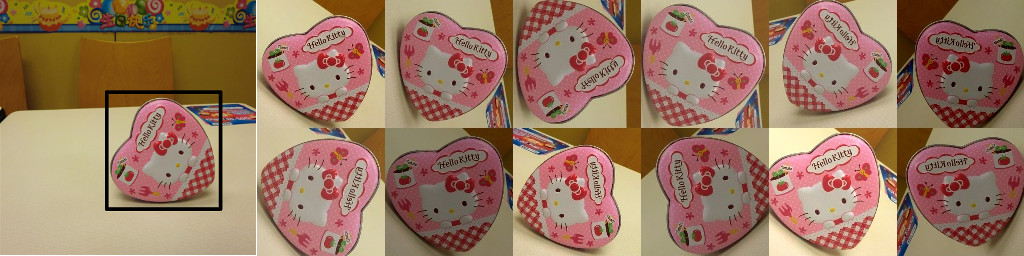
\includegraphics[width=1.0\textwidth]{focus/image_variations.jpg}
\label{fig:focus_variations}
\end{figure*}


In cropping an image to its object's bounding box, I use a uniform scaling - in order to ensure the entire object fits within this bounding box I fit a square around the bounding box in the cases where the bounding box is not square (I use square images as inputs to neural networks in this work).

I used data augmentation heavily to regularise the training in the form of random image transformations. Training images are randomly transformed using a set of parameters sampled from a normal distribution and shown in table~\ref{fig:focus_jitter}.  I use translations, rotation about the centre, scales (uniform and non uniform), and brightness and contrast adjustments. Testing images are re-sized and cropped in the same way (described below), but with no random transformations. An example of training data is given in figure~\ref{fig:focus_variations}.

\begin{table}[h]
  \centering
    \caption{Ranges of parameters used for image distortion }
    
  \begin{tabular}{ l  l }
    Parameter & Mean $ \pm $ Standard deviation \\
    \toprule
    scale (uniform) & $ 1 \pm 0.2 $  \\ 
    non uniform scale  & $ 1 \pm 0.2 $  \\ 
    rotation (degrees) & $ \pm 90 $ \\ 
    translation(x, y) (\% image size) & $ \pm 5 $ \\ 
    brightness (additive) & $ \pm 20 $ \\ 
    contrast (multiplicative) & $ 1 \pm 0.2 $ \\ 
    \bottomrule
  \end{tabular}
\label{fig:focus_jitter}
\end{table}


An affine transformation matrix $ (2 \times 3) $ is computed, firstly scaling the image to fit the bounding box region to match the network's input size, applying a set of random transformations as above, then cropping a rectangular region around the origin of the transformed image. I use OpenCV's \emph{warpAffine} function to perform this as a single step, avoiding artefacts from multiple image transformations (and also to avoid having to compute intermediate images with associated clipping issues).

\subsection{Datasets}

The RGB-D \cite{Lai2011} dataset contains turntable images with a fixed camera at 30 degrees, 45 degrees and 60 degrees of elevation. For evaluating instance recognition the 30 and 60 degree images are used for training, and the 45 degree images are used for testing. Bounding boxes are provided for each image (generated using depth information). The RGB-D dataset contains approximately 500 images (varying a little) for each instance, with 300 different object instances. I make no use of the depth images provided in the dataset.

The INSTRE \cite{Wang2015} aims to be a more diverse, better balanced dataset with more cluttered backgrounds than existing object instance recognition datasets. It improves on the RGB-D dataset in that the range of views are much more variety, both in the the types of object and the backgrounds (hand taken photos) compared with the turntable background. Bounding boxes are again provided. No standard test set is provided for the INSTRE dataset, so I take images of each object for testing, and use the remaining images for training at a ratio of $1:3$. The INSTRE dataset contains 200 classes of object, each with 100 images which have either been hand captured or picked. 

The INSTRE dataset contains unique challenges. A number of the objects are a little abstract, and include things like logos (e.g. one of the categories is KFC, which includes pictures of the building prominently showing the logo, as well as napkins containing the logo and pencil drawings). An example of a hard case is shown in figure~\ref{fig:focus_adidas}. Many categories feature objects rotated in numerous ways, with both landscape and portrait images, as well as many photos taken on angles with no alignment at all.

\section {Experiments}


\subsection {Experiment 1}

The first experiment compares the effect of focusing on the bounding box on classification accuracy. If there existed an oracle which could provide a bounding box estimate (or another model which could accurately give a bounding box estimate) - how much better is the network performance on cropped versus baseline (uncropped) images? I apply this cropping equally on test and training images.

For the RGB-D dataset, which for many of the objects only occupy a tiny space of the full image, I crop the inner centre to 40 percent of the image for the uncropped baseline. Otherwise, after scaling the original image to $ 64 \times 64 $ the smaller objects occupy only a few pixels, with the turntable and background being vastly bigger in scale. In order to see if the magnification from cropping to the bounding box was having an effect, I also ran the baseline at a higher resolution - but noticed little change in performance.


\begin{table}[h]
  \centering
    \caption{Cropped vs. uncropped images }
    
  \begin{tabular}{ l l l }
    
    Dataset & Image preparation & test set accuracy \\
    \toprule
    
    INSTRE & baseline &  65.3 \\
    INSTRE & bounds cropped & 89.0 \\
    
    RGB-D & centre cropped & 58.1 \\
    RGB-D & bounds cropped & 81.6 \\
    
    \bottomrule
  \end{tabular}
\label{fig:focus_crop}
\end{table}

The RGB-D results suggest over-fitting, with the training accuracy reaching almost 100 percent, yet generalising badly with the test set. The RGB-D images present a problem in that the test set (those images captured at 60 degrees elevation), is from a slightly different distribution from the training set (the images are captured at a constant level of elevation). Each image is also reasonably redundant due to being part of a video sequence. A potential solution to this is using a higher level of randomised non uniform scaling when training. The INSTRE images on the other hand have no systematic difference between training and test images and also cover a much greater intra-object variation but do not show the same kind of over-fitting.

It is clear that focusing on the bounding box has a large impact on the performance of the classification, with both RGB-D and INSTRE classification improved when trained and tested on images cropped to the bounding box. Given this is the case, I seek to discover exactly why. Which property is it that enables effective classification using this kind of CNN model? Is it the magnification of the object after cropping an image to the bounding box, or removing the distracting background? (It is clear the object is much larger in pixels after the resulting image is scaled to match the CNN input size). Alternatively, is it the centring of the object, suggesting the translation invariance of the CNN is not as general as is widely assumed?


\subsection {Experiment 2}

\begin{figure*}[t]
    \caption{Examples of cropping for context}
\centering
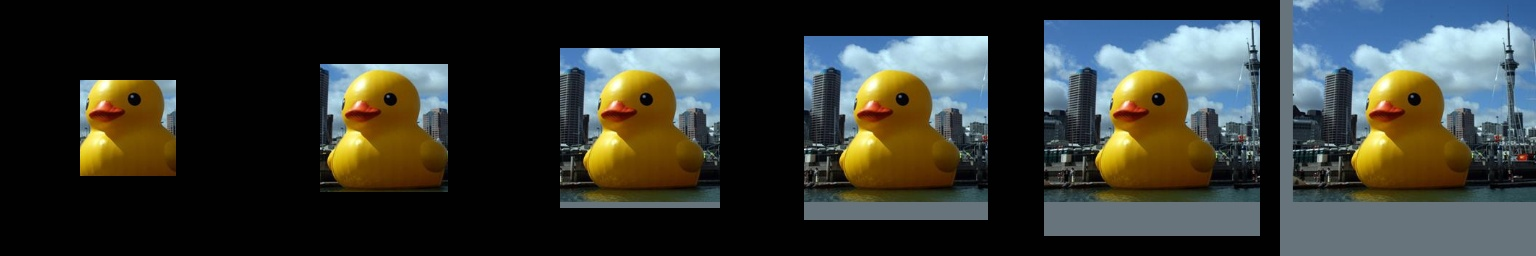
\includegraphics[width=1.0\textwidth]{focus/enlarge.jpg}
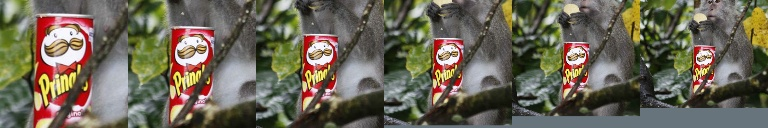
\includegraphics[width=1.0\textwidth]{focus/shrink.jpg}
\label{fig:focus_context}
\end{figure*}




\begin{figure}[h]
    \caption{Context in image classification vs. test set accuracy}
\centering
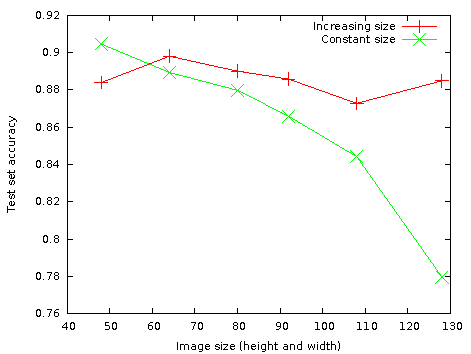
\includegraphics{focus/graph.pdf}
\label{fig:focus_exp2}
\end{figure}

For the second experiment I explore how including context changes the performance. I do this in two ways. Firstly by fixing the pixel size of our object and including more context by using a larger input image to the model. Secondly by fixing the size of the input to the network and including the same context, where the object is scaled down to accommodate.

In the first case I scale the object bounding box to $ 64 \times 64 $ and set this as the base scale, each larger size includes proportionally more context where the object remains a constant size in pixels. In the second case I use a fixed image size of $ 64 \times 64 $, using the same image context for each size as the first case, causing the object to be  scaled to be relatively smaller. 

The architecture of the network is mostly unmodified (each image output within the hidden convolutional layers in the network is of a larger dimension). The number of parameters is constant for the convolutional layers, but the first fully connected layer contains a larger number of inputs to cope with the extra outputs from the convolutional part. The differences can be seen in table~\ref{fig:focus_sizes}.


\begin{table}[h]
  \centering
    \caption{Example output sizes for input dimensions }
\begin{tabular}{ l l l } 
 
 \toprule
 Input image size & Convolution outputs & Flattened size \\
 \toprule
 
 $ 48 \times 48 \times 3 \rightarrow $ & $ 1\times1\times144 \rightarrow $ & 144 \\
 $ 64 \times 64 \times 3 \rightarrow $ & $ 2\times2\times144 \rightarrow $ & 576 \\
 $ 108 \times 108 \times 3 \rightarrow $ & $ 3\times3\times144 \rightarrow $ & 1296 \\
 $ 128 \times 128 \times 3 \rightarrow $ & $ 4\times4\times144 \rightarrow $ & 2304 \\
 
\end{tabular}
\label{fig:focus_sizes}
\end{table}

I can see from the data shown in figure~\ref{fig:focus_exp2} that performance is relatively constant where the scale of the object is fixed. Adding context neither gives a performance boost nor hinders recognition (only takes longer to train). Where context is added at the expense of the object scale I can see that at the higher levels the test accuracy drops.


\subsection {Experiment 3}

Given the results from experiment~2, it seems that reducing the scale of the object (in pixel size) causes a degradation of the performance. Experiment~1 shows that the unmodified INSTRE images are still much more difficult to classify for a CNN. Experiment 2 normalises scales between objects (for example.e. the Statue of Liberty becomes the same size in terms of image pixels as a can of cola). For experiment 3 I use the bounding box to centre the object, but leave the scale unmodified.


\begin{table}[h]
  \centering
    \caption{Effect of input size and centring}
    
  \begin{tabular}{ l l l l }
    
    Dataset & Input size & Test set accuracy \\
    \toprule
    
    INSTRE &  $ 64 \times 64 $ & 65.3 \\
    INSTRE &  $ 128 \times 128 $  & 71.7 \\
    INSTRE &  $ 192 \times 192 $  & 76.0 \\
    
    \toprule
    INSTRE (centred) &  $ 64 \times 64 $ & 71.6 \\
    INSTRE (centred) &  $ 128 \times 128 $  & 80.6 \\
    INSTRE (centred) &  $ 192 \times 192 $  & 84.2 \\
    
    
    
    \bottomrule
  \end{tabular}
\label{fig:focus_input_size}
\end{table}



I can see from this experiment that both increasing magnification, as well as centring the object both give significant accuracy boosts, not to the same level as cropping to the bounding box, but close. Perhaps even larger magnification would be fruitful. 

The fact that centring the object makes such a difference is surprising, given the translation invariance of the CNN architecture, however it is not clear exactly how much a CNN is translation invariant (even though I can see that the filters used in a convolution step are clearly translation invariant - it is not obvious that the network as a whole possesses such properties). A recent study attempting to quantify this translation invariance \cite{EricKauderer-Abrams2016} suggests the architecture, and data augmentation are both important here. 


\subsection {Failure cases - discussion}


\begin{figure*}[t]
    \caption{Example of one hard case in the INSTRE dataset}
\centering
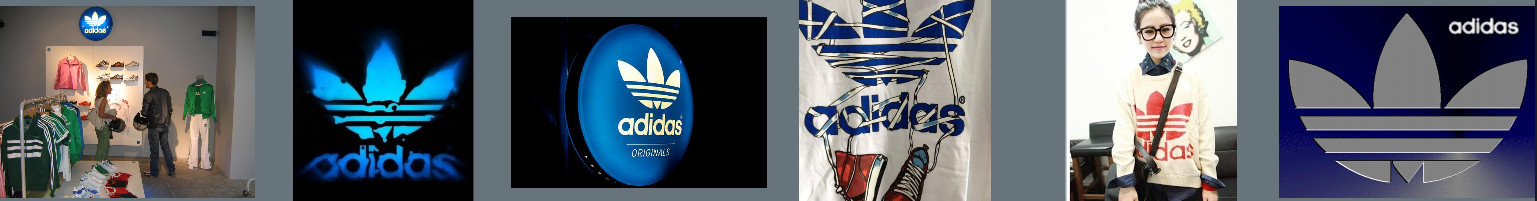
\includegraphics[width=1.0\textwidth]{focus/adidas.jpeg}
\label{fig:focus_adidas}
\end{figure*}



\begin{table}[h]
  \centering
    \caption{Worst categories in testing }
  \begin{tabular}{ l l }
  wangzai & 46.6 \\
  einstein bros & 46.6\\
  Manneken Pis & 45.4\\
  mastermind JAPAN & 45.1\\
  clapperboard & 43.2\\
  Che Guevara & 38.2\\
  coca cola & 33.3\\
  Paul Frank Julius & 32.4\\
  Kung Fu Panda & 24.0\\
  Adidas Originals & 17.2\\
    \bottomrule
  \end{tabular}
\label{fig:focus_failure}
\end{table}

It can be seen in figure~\ref{fig:focus_failure}, that many of the worst performing object classes were those which are somewhat abstract, for example logos which were stylistically the same logo but appeared visually quite different with different colours, materials and occurring in very different contexts. An example is shown in figure~\ref{fig:focus_adidas} for the ``Adidas Originals'' object.

\section{Conclusion}

I found that CNN classification on the cropped bounding box regions is much more accurate than classification of whole images. Both magnification and centring of the object in question seem to have a strong effect (which is somewhat surprising, given the translational invariance properties of CNN models). In the experiments I performed, including context in the input images was only useful if it does not come at the expense of minifying the object (reducing its pixel size) to be classified.

I conclude that in order to perform quality instance recognition using \gls{CNN}s for classification, it would be a strong advantage to first localise the region of interest, and then focus on the region of interest.  In future I will both further investigate why I see the results above, and at the same time peruse how focus methods can be used to improve instance recognition. The failure modes in unfocused image classification is also of interest for understanding in more depth our observations. For the INSTRE data set, the more abstract categories were among those which failed to generalise well, and RGB-D dataset simply over-fit badly.

I will explore bounding box regression as is used in many object detection methods, as well as rotation regression for the purposes of aligning input images to a canonical orientation. One difficulty with using regression is the requirement that your training data requires annotation, making its use in practice more expensive to obtain. Alternatives include using using external data, and using methods of semi-automated segmentation (for example using a green screen). Alternatively, the use of Spatial Transformer networks is interesting as it requires no such annotation, and jointly learns the focus method with the classifier.






\chapter{Object Recognition by Stochastic Metric Learning}
\label{chap:metric} 

Descriptors extracted from deep neural networks have been shown to be very discriminative. Networks such as those trained on the large, very general ImageNet dataset have been used to extract descriptors which can then be used robustly for a variety of image classification tasks. Such retrieval systems utilise feature locality, for example, Approximate Nearest Neighbour. The goal is to use such descriptors as part of a large scale object instance recognition and retrieval system. I propose using deep nonlinear metric learning on Convolutional Neural Networks to learn features with good locality. In particular, I worked with two related methods, \gls{NCA} and the related \gls{MEGM}.

I utilise a nonlinear form of \gls{MEGM} as an alternative to \gls{NCA} and propose some stochastic sampling methods to apply these batch learning methods to larger datasets with mini-batch \gls{SGD}. On a larger scale, I found the methods challenging to train, failing to converge or generalising poorly depending on the training method or parameters. This led to returning to a smaller dataset and examining the factors which lead to good generalisation with this form of training.
  
Surprisingly, on a small subset of the RGB-D dataset, stochastic sampling methods generalised much better with small batch sizes (they acted as a form of regularisation). When trained with larger batches, or as a full batch, the dataset was overfitted. Given the correct parameters, extracted descriptors performed well at the Nearest Neighbour task and exceeded the performance of those extracted by applying standard supervised training.

\section{Introduction}

Deep convolutional neural networks, in combination with modern \gls{GPU}s and large image datasets, have shown strong performance on image classification tasks \cite {Krizhevsky2012}, and have been applied to related problems such as object detection \cite{Sermanet2013}, image segmentation \cite{Masci2013} and image retrieval \cite{Razavian2014}.

\subsection {Descriptors from Deep Neural Networks}

Using descriptors, derived from the hidden layers of neural networks trained for classification, for the purpose of other learning tasks, is a relatively new idea. These descriptors have been shown to be robust even for quite unrelated tasks \cite{Donahue2014,Razavian2014}. The ImageNet dataset \cite{Krizhevsky2012} is a popular source for pre-training, and pre-trained models exist such as the OverFeat network \cite{Sermanet2013} or the DeCAF feature extractor \cite{Donahue2014}). 

A standard technique in training a \gls{CNN} is to augment the dataset by applying transformations, as more data typically gives better generalisation. In \cite{Dosovitskiy2013}, a \gls{CNN} was trained on single images which were warped in many different ways. Features obtained from the network were then used in popular classification benchmarks achieving good results. For many years local image descriptors such as \gls{SIFT} \cite{Lowe2004} have been used for matching and indexing images.  A recent comparison \cite{Fischer2014} (though perhaps not a fair one) showed that using a \gls{CNN} for matching tasks performed better than \gls{SIFT} by a margin similar to the improvement given by \gls{SIFT} to raw pixel data.


The final layer of a standard deep neural network, as used in supervised classification, consists of a set of linear classifiers, such as those descriptors that are suitable for classification using other linear classifiers, for example, \gls{SVM}s. Nearest Neighbor suffers from high dimensionality and noisy or irrelevant dimensions, so the descriptors produced by a CNN may not be suitable for comparison by distance. For that reason, I have looked towards metric learning to directly optimise the descriptors for Nearest Neighbor classification. 


\subsection {Deep Metric Learning}


Metric learning has often been used for object recognition and image classification \cite{Hadsell2006,Min2009} (and many others), and especially face recognition, for example \cite{Kostinger2012}. Although most efforts have often focused on Mahalanobis distance metric learning (a form of distance metric learning linear transformation), deep metric learning has had some attention \cite {Salakhutdinov2007a,Min2009,Weston2009,Min2010}. At the expense of a much larger computation cost, deep metric learning has been shown to perform much better than its linear counterparts. Gradients from metric learning are used to drive \gls{SGD} on a deep \gls{CNN}. 

Functions for metric learning often focus on pairs or triples, using siamese networks where parameters are shared between two or three branches of identical networks. This method generalises this to multiple examples at a time.

\subsection {Training}

Metric learning comes with its own set of challenges, and it has often been formulated as a batch training method because each example potentially interacts with every other example. In practice, descriptors from examples far apart do not interact with each other at all, so approximations can be made, as discussed later. High dimensional spaces from feature vectors can face issues, namely the ``curse of dimensionality''. In high dimensional spaces, evenly spaced points (descriptors) increase in the number of neighbours with increased dimension. 

The interaction between points decays with distance (for example, exponentially with \gls{NCA}). I can use approximations around the local neighbourhood of examples which can be used to create a \gls{SGD} training procedure. Using an approximation to the nearest $ k $, neighbours is an approach seen in \cite{Mensink2012,Zaidi2011} (among many). Clustering (amongst other sampling methods) is discussed in  \cite{Oneat2011} such as Farthest Point or Random Projection clustering, but the downside of such clustering is that it is hard to control the size of a batch. 

Many training methods focus on the interaction between pairs of (similar/dissimilar) examples or triples (example, more similar, less similar), for example, DrLIM \cite{Hadsell2006} where a spring analogy is used to create an attraction between similar pairs and repulsion between dissimilar pairs. The advantage of pairwise methods is that they can be used with the weaker labelling of similar/dissimilar (as opposed to category label).

\section {Deep Metric Learning}

A deep neural network (in this case a \gls{CNN}) is used to embed images into a lower dimensional space, creating descriptors which can be compared with their Euclidean distance (and classified with nearest neighbour) where the Euclidean distance of the raw pixels is both computationally expensive and not a good measure of the distance of the semantic similarity of image content. 

I examine non-linear versions of two methods, \gls{NCA} \cite{Goldberger2004} and the closely related but less well known \gls{MEGM} \cite {Zaidi2011}. \gls{NCA} optimises a continuous version of the \gls{LOO} performance, and it uses a softmax over weights which decay exponentially with distance. The \gls{NCA} score can be interpreted as the probability that a descriptor will pick another descriptor of the correct class as its nearest neighbour. 

The probability, $ p_{ij} $, of one descriptor selecting another descriptor as its neighbour, is defined as a softmax function over weights $W_ij$. The indexes $ i $ and $ j $ refer to input examples $x_i$ and $x_j$, and corresponding vector valued output of a \gls{CNN} $f(x_i)$ and $f(x_j)$ which are the descriptor vectors.

\begin{equation}
\label{eq:nca_prob_pair}
p_{ij} =  \frac {W_{ij}} {\sum_{k \neq i}{W_{ik}}}g
\end{equation}

Then the total probability, $ p_i $, of a point selecting any neighbour with another with its \emph{correct} class is defined as the sum of those neighbour probabilities $p_{ij}$ which have the same class:

\begin{equation}
\label{eq:nca_prob}
p_{i} =  \sum_{j:c_j = c_i}{p_{ij}}
\end{equation}

Where $ C_i $ is the class label of example $ i $. A Gaussian kernel is used for the weighting as \cite{Zaidi2011} do. 

\begin{equation}
 \label{eq:gaussian_kernel}
W_{ij} = exp(\frac{-\lVert f(x_i) - f(x_j) \rVert^2_2 }{2\sigma^2}), \space W_{ii} = 0
\end{equation}


The function to be maximised is the sum of the probabilities of all descriptors being correctly classified.

\begin{equation}
\label{eq:nca_loss}
\mathcal{E}_{nca} =  \sum_i {p_i}
\end{equation}

Where \gls{NCA} optimises directly on the probability $ p_{i} $ above, \gls{MEGM} instead computes for each class $ \hat{y_{ti}} $ as a prediction that a descriptor will take class $ t $, where the only difference is that $ c_j = t $ as opposed to $ c_j = c_i $:

\begin{equation}
\label{eq:megm_pred}
\hat{y_{ti}} = \frac{\sum_{j:c_j = t}W_{ij}}{\sum_{k \neq i}{W_{ik}}}
\end{equation}

The prediction $ \hat{y_{ti}} $ can then be compared with $ y_{ti} $ (1 where $ t = c_i $, 0 otherwise), and it then minimises the \gls{MSE} between prediction and true class label:

\begin{equation}
\label{eq:megm_loss}
\mathcal{E}_{megm} =  \sum_i\sum_t{(y_{ti} - \hat{y_{ti}})^2}
\end{equation}

Intuitively \gls{MEGM} can be seen to penalise the case where two classes compete for the same region,  more so than when one class competes against examples of many different classes, whereas \gls{NCA} would treat the two cases approximately equally. These loss functions can be used to drive gradient descent on a \gls{CNN} by standard back-propagation. The derivative for \gls{MEGM} is shown in the appendix, section~\ref{sec:appendix}.

The gradient is computed over the outputs of each mini-batch and apply back-propagation to find the derivative with respect to the weights of the network. It can be noted that the output and derivative for \gls{MEGM} is more expensive to compute because of the additional per class summation, so it would not be suitable with an extremely large number of classes. In practice, a large number of the terms can be factored out and pre-computed, as well as computing the difference summations in terms of matrix multiplication.

Note the parameter $ \sigma $ was not in the original \gls{NCA}, and is initialised to the average distance to the nearest neighbours of the initial descriptor output before training. It is used to prevent the weights initialising to zero when the distance between descriptors is large.


The parameter $\alpha $ controls the trade-off. When $ \alpha \mathcal{E}_{mse} > \mathcal{E}_{nca} $ the descriptors all collapse into the same point.


\section{SGD for metric learning}

The main proposal is in using mini-batch \gls{SGD}, and applying it to metric learning methods which have been designed as batch learning methods. Metric learning as shown above as a batch method, scales at $ O(n^2) $ for $ n $ examples. Given that the desire to apply these approaches to large datasets containing hundreds of thousands or millions of images, I am forced to consider approximations. The typical method for training a \gls{CNN} on large numbers of images is using \gls{SGD}, because it is fast, simple and scales to handle large datasets easily. 

The most obvious approximation is to truncate the influence to the nearest $ k $ neighbours as the weight exponentially decays with the square distance. It is hypothesised this would lead to the best approximation, however, there are many ways of truncating the neighbourhoods. This lends itself to clustering methods and is more complicated than the alternative, which is to sample batches randomly but uses a large enough batch to include several examples of each class.

I propose the following approaches for sampling batches for \gls{SGD}:

\begin{enumerate}
\item {\bf Random shuffled batches} \par
 Randomly shuffle the dataset and divide it up into batches of a fixed size, which is exactly how batches would normally be selected for supervised learning. Each batch contains (almost certainly) different numbers of examples from each class.
 \item {\bf Stratified random batches}  \par
 Pick batches by selecting a number of examples from each class, to ensure the same number of examples of each class are represented in each batch.   
 \item {\bf K-neighbourhoods around random points}  \par
 Before each training epoch, run the model forward through the training set to obtain descriptors for each example. Select N examples at random and pick the batch as the batch sized neighbourhood (in descriptor space) of each selected example.
\end {enumerate}


\subsection {Issues of Scale}

The parameter $ \sigma $ is optional in theory, as the scale can be factored into the final fully connected weight matrix (or previous layers).  I make use of $ \sigma $ for numerical stability upon initialisation, and during training the density of points adjusts itself to fit this parameter. It can also be observed that for different values of $ \sigma $, that the distance between descriptors adjusts themselves to fit the new parameter over a few iterations of training.


\subsection {Adding Mean Square Error}

I experimented with adding the square distance between members of the same class, as a means of adding some bias to the loss functions after suspecting that metric learning methods described above were overfitting, to force the output distribution to be more simple. 

\begin{equation}
\label{eqn:mse}
\mathcal{E}_{mse} = \sum_i{ \sum_{j:j_c = i_c}  \frac {{\lVert f(x_i) - f(x_j) \rVert^2_2}} {\sigma^2} }
\end{equation}

\begin{equation}
\label{eqn:mse_total}
\mathcal{E}_{total} =  \mathcal{E}_{nca} + \alpha \mathcal{E}_{mse}
\end{equation}


\subsection {kNN implementation}

I use a brute force \gls{KNN} algorithm written in CUDA \cite{Garcia2008} for the \gls{GPU}, computing the distance matrix using matrix multiplication followed by using an insertion sort to select the $ k $ neighbours of lowest distance. This approach is not scalable to large datasets, and smarter clustering algorithms will eventually need to be used; however, the time for evaluating \gls{KNN} on the datasets I experimented with, are still dominated by the cost of computing descriptors from examples. 


\section {CNN architecture}


\begin{figure}[ht]
\centering
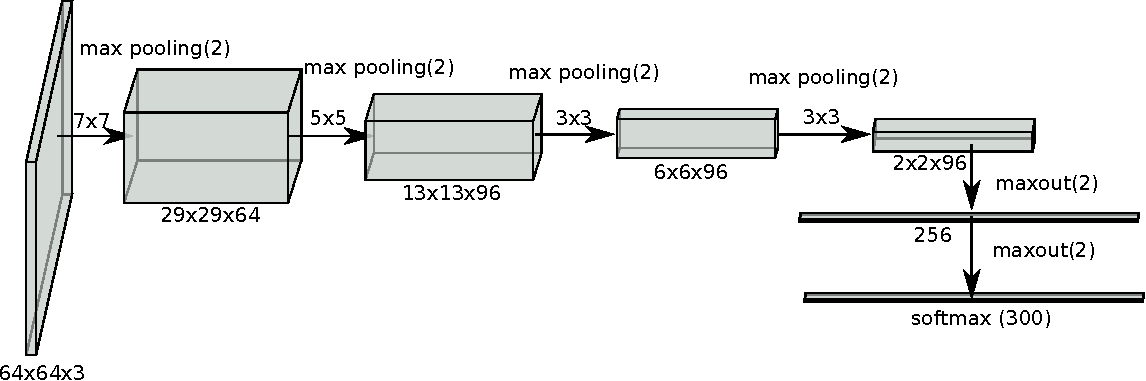
\includegraphics[width=1\textwidth]{metric_learning/convnet.pdf}
\caption{Convolutional network configuration used for $64\times64$ RGB images with supervised learning.}
\label{fig:metric_convnet}
\end{figure}

I used a simple convolutional neural network of six layers, with four layers of convolution and max-pooling using rectified linear activation functions, with two fully connected layers using Maxout \cite{Springenberg2013} units as an activation method, shown in Figure~\ref{fig:metric_convnet}. Dropout \cite{HintonDropout} with a rate of $ 0.5 $ is used when training on inputs to the two fully connected layers. For metric learning, the last linear layer and softmax are removed, leaving four convolutional layers and a single fully connected layer giving descriptors of size $ 256 $.

Dropout and Maxout have been shown to be beneficial in a supervised learning scenario for the purposes of regularisation. In the standard supervised training scenario, Dropout is of practical use because it (to some degree) prevents overfitting, and mostly does away with the need for early stopping. However, I found that it interfered with generalisation when used with metric learning approaches.

\subsection {Data augmentation}

\begin{figure}[h]
\centering
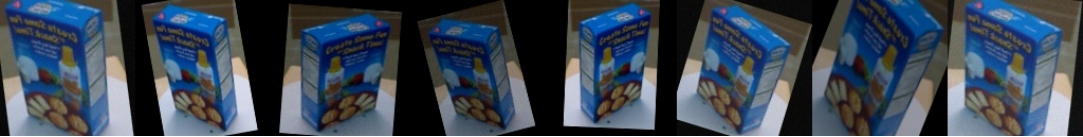
\includegraphics[width=1\textwidth]{metric_learning/augmentation.png}
\caption{Example of image distortions resulting from transformations of a single source image}
\label{fig:metric_augmentation}
\end{figure}


In all cases, I used randomised data augmentation of the test set by applying random distortions to ensure the network never saw exactly the same image twice, and to increase its tolerance to small changes in lighting, translation and rotation. The parameters of the data augmentation can be seen in Figure~\ref{fig:metric_permute}. Without the data augmentation, supervised training produces substantially worse generalisation than without, in both supervised and metric learning approaches. In all experiments, testing was performed on non-augmented images and trained with augmented images.

\begin{table*}
  \centering
    \caption{Ranges of parameters used for image augmentation }

  \begin{tabular}{ l  l }
    \toprule
    scale (uniform) & $ 1 \pm 0.2 $  \\ 
    squash  & $ 1 \pm 0.2 $  \\ 
    rotation (rads) & $ \pm \frac{\pi}{16} $ \\ 
    translation(x, y) (\% image size) & $ \pm 5 \% $ \\ 
    brightness (additive) & $ \pm 20 \% $ \\ 
    contrast (multiplicative) & $ 1 \pm 0.2 \% $ \\ 
    gaussian pixel noise & $ \sigma = 2 \pm 2 $  \\ 
    flip horizontal (probability) & $ 0.5 $ \\ 
    \bottomrule
  \end{tabular}
\label{fig:metric_permute}
\end{table*}

\subsection {Dataset}

\begin{figure}[h]
\centering
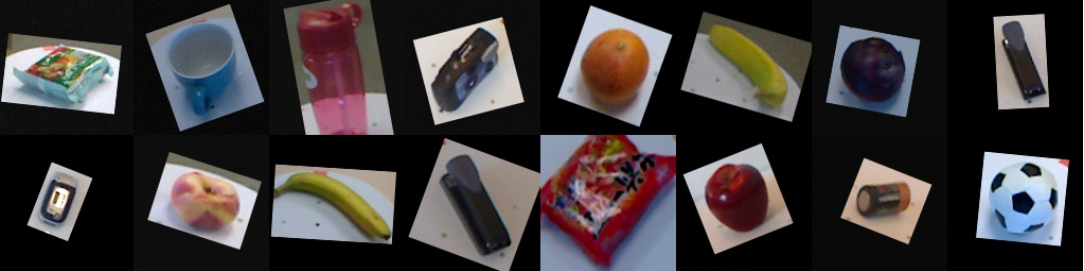
\includegraphics[width=1\textwidth]{metric_learning/objects.png}
\caption{Samples of images of different objects used in training}
\label{fig:metric_dataset}
\end{figure}

I experimented with the University of Washington RGB-D dataset primarily because it has a standard test set for instance recognition and a large number of published results. It contains 300 objects from 50 classes. Each object has three sequences of rotations at 30, 45 and 60 degrees elevation. Each rotation sequence contains approximately 150 images. For instance recognition, the sequence at 30 and 60 degrees are used for training, and the sequence at 45 degrees is used for testing. 

A cut-down version of the RGB-D dataset is used for a number of experiments, with 50 objects and 100 images of each object to train on, and 50 images per object to test. The images were randomly selected.

The resolution of $ 64\times64 $ on the RGB-D images is used, with the cropped version of the images. The procedure for resizing is to load all of the images in a sequence and if any image is at a higher resolution than $ 72\times72$, I resize the image to $ 72\times72 $. The same factor scales all other images in the sequence. The images are then augmented (see Figure~\ref{fig:metric_permute}) and finally centred (modulo translation) on a blank image at  $ 64\times64 $.


\section {Experiments}

In all cases (unless otherwise specified), I use a mini-batch size of 256, with standard \gls{SGD} learning rate set to $ 10^{-2} $ for supervised learning, and $ 10^{-5} $ for metric learning methods. I experimented with other learning rates for metric learning, and in some cases, a lower learning rate of $ 10^{-6} $ was used when the higher rate caused divergence.

I manually divided the training rate by a factor of 10 when the training set accuracy plateaus for supervised learning. Supervised learning methods greatly benefit from reducing the learning rate after time. However, there was no noticable benefit to the metric learning methods. I stopped metric learning methods at 70 epochs or earlier, if they were not converging. Overall, \gls{MEGM} gave similar, but slightly better test set accuracy than \gls{NCA}, and most experiments used \gls{MEGM} for consistency.


\subsection{Overall Comparison}

I compared the testing classification error between methods, and the final accuracy is reported as the test set classification accuracy average over the last 5 iterations. Test set accuracy is percentage accuracy. For metric learning, the class chosen is the most common class in $k = 5$ nearest neighbours.


\begin{table*}[ht]

\centering
  \caption{Summary of training methods}

  \begin{tabular}{  l l  l  l l l }
  
    \toprule
    method &  sampling & batch  & test accuracy &  train epochs \\  \hline
    \bf{Initialisation} & &  &  $ 64.0  $ & 0  &  \\  
    \hline
    
    \bf{Supervised} & & 256 &  $ 90.6  $ & 40  &  \\  
     & 5NN  &  &  $ 89.0  $ & 40 &  \\  
     \hline
    
    \bf{NCA} &  & batch &  $  71.2  $ &  50  & \\
     & random & 256 & $  94.0  $ & 70 & \\
    
    \hline
    
    \bf{MEGM} &  & batch  &  $  74.4  $ &  50  & \\
     & random & 128 &  $  95.0  $ &  70  & \\     
     &  & 256 & $  90.5  $ &  70 & \\  
     &  & 512 & $  81.4  $ &  70 & \\
    
    \hline
    \bf{MEGM} & stratified & 128 & $  {\bf 95.4 }  $ & 70 & \\  
    
     &  & 256 & $  94.6  $ & 70 & \\  
     &  & 512 & $  87.1  $ & 70 & \\  

     \hline
     
    \bf{MEGM} & neighbourhoods & 256 & $  80.4  $ & 70  & \\
    
    \hline
    
    \bf{MEGM + MSE} & stratified & 128 & $  {\bf 95.3 }  $ & 70  & \\

      \bottomrule
    
    \end{tabular}
\label{fig:metric_summary}
\end{table*}



I sought to compare the sampling approximation to the full batch (as opposed to mini-batch) method. As a batch method, \gls{SGD} is not the ideal training method. It was surprising to see that despite the loss function smoothly decreasing (as can be
seen in Figure~\ref{fig:metric_megm_test}), training failed to generalise well to the training set (Figure~\ref{fig:metric_megm_loss}).
I anticipated that the batch metric learning methods would work best as a batch
method or with larger batches (as closer approximations to the batch method).
It is seen that is not the case, and both the batch method and \gls{SGD} with the larger batch size (512) both failed to generalise well. The same pattern occurred for \gls{NCA}, as well as using the stratified sampling method. The reason for such overfitting is, I believe, that the two metric learning methods have not enough bias to force the network to learn something. \gls{NCA} allows highly complex and multi-modal distributions with many local minima, which provided the local neighbourhood structure fits, are not penalised by its loss function. Smaller batch sizes, however, act as a regularisation, forcing the descriptor outputs into a simpler form.



\begin{figure}[ht]
   \begin{tikzpicture}[gnuplot]
%% generated with GNUPLOT 4.6p1 (Lua 5.1; terminal rev. 99, script rev. 100)
%% Thu 31 Jul 2014 02:53:39 NZST
\gpsolidlines
\path (0.000,0.000) rectangle (12.700,7.620);
\gpcolor{color=gp lt color axes}
\gpsetlinetype{gp lt axes}
\gpsetlinewidth{1.00}
\draw[gp path] (1.504,0.985)--(12.147,0.985);
\gpcolor{color=gp lt color border}
\gpsetlinetype{gp lt border}
\draw[gp path] (1.504,0.985)--(1.684,0.985);
\draw[gp path] (12.147,0.985)--(11.967,0.985);
\node[gp node right] at (1.320,0.985) { 0};
\gpcolor{color=gp lt color axes}
\gpsetlinetype{gp lt axes}
\draw[gp path] (1.504,1.556)--(12.147,1.556);
\gpcolor{color=gp lt color border}
\gpsetlinetype{gp lt border}
\draw[gp path] (1.504,1.556)--(1.684,1.556);
\draw[gp path] (12.147,1.556)--(11.967,1.556);
\node[gp node right] at (1.320,1.556) { 0.1};
\gpcolor{color=gp lt color axes}
\gpsetlinetype{gp lt axes}
\draw[gp path] (1.504,2.127)--(12.147,2.127);
\gpcolor{color=gp lt color border}
\gpsetlinetype{gp lt border}
\draw[gp path] (1.504,2.127)--(1.684,2.127);
\draw[gp path] (12.147,2.127)--(11.967,2.127);
\node[gp node right] at (1.320,2.127) { 0.2};
\gpcolor{color=gp lt color axes}
\gpsetlinetype{gp lt axes}
\draw[gp path] (1.504,2.698)--(12.147,2.698);
\gpcolor{color=gp lt color border}
\gpsetlinetype{gp lt border}
\draw[gp path] (1.504,2.698)--(1.684,2.698);
\draw[gp path] (12.147,2.698)--(11.967,2.698);
\node[gp node right] at (1.320,2.698) { 0.3};
\gpcolor{color=gp lt color axes}
\gpsetlinetype{gp lt axes}
\draw[gp path] (1.504,3.269)--(12.147,3.269);
\gpcolor{color=gp lt color border}
\gpsetlinetype{gp lt border}
\draw[gp path] (1.504,3.269)--(1.684,3.269);
\draw[gp path] (12.147,3.269)--(11.967,3.269);
\node[gp node right] at (1.320,3.269) { 0.4};
\gpcolor{color=gp lt color axes}
\gpsetlinetype{gp lt axes}
\draw[gp path] (1.504,3.840)--(12.147,3.840);
\gpcolor{color=gp lt color border}
\gpsetlinetype{gp lt border}
\draw[gp path] (1.504,3.840)--(1.684,3.840);
\draw[gp path] (12.147,3.840)--(11.967,3.840);
\node[gp node right] at (1.320,3.840) { 0.5};
\gpcolor{color=gp lt color axes}
\gpsetlinetype{gp lt axes}
\draw[gp path] (1.504,4.411)--(12.147,4.411);
\gpcolor{color=gp lt color border}
\gpsetlinetype{gp lt border}
\draw[gp path] (1.504,4.411)--(1.684,4.411);
\draw[gp path] (12.147,4.411)--(11.967,4.411);
\node[gp node right] at (1.320,4.411) { 0.6};
\gpcolor{color=gp lt color axes}
\gpsetlinetype{gp lt axes}
\draw[gp path] (1.504,4.982)--(12.147,4.982);
\gpcolor{color=gp lt color border}
\gpsetlinetype{gp lt border}
\draw[gp path] (1.504,4.982)--(1.684,4.982);
\draw[gp path] (12.147,4.982)--(11.967,4.982);
\node[gp node right] at (1.320,4.982) { 0.7};
\gpcolor{color=gp lt color axes}
\gpsetlinetype{gp lt axes}
\draw[gp path] (1.504,5.553)--(9.759,5.553);
\draw[gp path] (11.963,5.553)--(12.147,5.553);
\gpcolor{color=gp lt color border}
\gpsetlinetype{gp lt border}
\draw[gp path] (1.504,5.553)--(1.684,5.553);
\draw[gp path] (12.147,5.553)--(11.967,5.553);
\node[gp node right] at (1.320,5.553) { 0.8};
\gpcolor{color=gp lt color axes}
\gpsetlinetype{gp lt axes}
\draw[gp path] (1.504,6.124)--(9.759,6.124);
\draw[gp path] (11.963,6.124)--(12.147,6.124);
\gpcolor{color=gp lt color border}
\gpsetlinetype{gp lt border}
\draw[gp path] (1.504,6.124)--(1.684,6.124);
\draw[gp path] (12.147,6.124)--(11.967,6.124);
\node[gp node right] at (1.320,6.124) { 0.9};
\gpcolor{color=gp lt color axes}
\gpsetlinetype{gp lt axes}
\draw[gp path] (1.504,6.695)--(12.147,6.695);
\gpcolor{color=gp lt color border}
\gpsetlinetype{gp lt border}
\draw[gp path] (1.504,6.695)--(1.684,6.695);
\draw[gp path] (12.147,6.695)--(11.967,6.695);
\node[gp node right] at (1.320,6.695) { 1};
\gpcolor{color=gp lt color axes}
\gpsetlinetype{gp lt axes}
\draw[gp path] (1.504,0.985)--(1.504,6.695);
\gpcolor{color=gp lt color border}
\gpsetlinetype{gp lt border}
\draw[gp path] (1.504,0.985)--(1.504,1.165);
\draw[gp path] (1.504,6.695)--(1.504,6.515);
\node[gp node center] at (1.504,0.677) { 0};
\gpcolor{color=gp lt color axes}
\gpsetlinetype{gp lt axes}
\draw[gp path] (3.024,0.985)--(3.024,6.695);
\gpcolor{color=gp lt color border}
\gpsetlinetype{gp lt border}
\draw[gp path] (3.024,0.985)--(3.024,1.165);
\draw[gp path] (3.024,6.695)--(3.024,6.515);
\node[gp node center] at (3.024,0.677) { 10};
\gpcolor{color=gp lt color axes}
\gpsetlinetype{gp lt axes}
\draw[gp path] (4.545,0.985)--(4.545,6.695);
\gpcolor{color=gp lt color border}
\gpsetlinetype{gp lt border}
\draw[gp path] (4.545,0.985)--(4.545,1.165);
\draw[gp path] (4.545,6.695)--(4.545,6.515);
\node[gp node center] at (4.545,0.677) { 20};
\gpcolor{color=gp lt color axes}
\gpsetlinetype{gp lt axes}
\draw[gp path] (6.065,0.985)--(6.065,6.695);
\gpcolor{color=gp lt color border}
\gpsetlinetype{gp lt border}
\draw[gp path] (6.065,0.985)--(6.065,1.165);
\draw[gp path] (6.065,6.695)--(6.065,6.515);
\node[gp node center] at (6.065,0.677) { 30};
\gpcolor{color=gp lt color axes}
\gpsetlinetype{gp lt axes}
\draw[gp path] (7.586,0.985)--(7.586,6.695);
\gpcolor{color=gp lt color border}
\gpsetlinetype{gp lt border}
\draw[gp path] (7.586,0.985)--(7.586,1.165);
\draw[gp path] (7.586,6.695)--(7.586,6.515);
\node[gp node center] at (7.586,0.677) { 40};
\gpcolor{color=gp lt color axes}
\gpsetlinetype{gp lt axes}
\draw[gp path] (9.106,0.985)--(9.106,6.695);
\gpcolor{color=gp lt color border}
\gpsetlinetype{gp lt border}
\draw[gp path] (9.106,0.985)--(9.106,1.165);
\draw[gp path] (9.106,6.695)--(9.106,6.515);
\node[gp node center] at (9.106,0.677) { 50};
\gpcolor{color=gp lt color axes}
\gpsetlinetype{gp lt axes}
\draw[gp path] (10.627,0.985)--(10.627,5.283);
\draw[gp path] (10.627,6.515)--(10.627,6.695);
\gpcolor{color=gp lt color border}
\gpsetlinetype{gp lt border}
\draw[gp path] (10.627,0.985)--(10.627,1.165);
\draw[gp path] (10.627,6.695)--(10.627,6.515);
\node[gp node center] at (10.627,0.677) { 60};
\gpcolor{color=gp lt color axes}
\gpsetlinetype{gp lt axes}
\draw[gp path] (12.147,0.985)--(12.147,6.695);
\gpcolor{color=gp lt color border}
\gpsetlinetype{gp lt border}
\draw[gp path] (12.147,0.985)--(12.147,1.165);
\draw[gp path] (12.147,6.695)--(12.147,6.515);
\node[gp node center] at (12.147,0.677) { 70};
\draw[gp path] (1.504,6.695)--(1.504,0.985)--(12.147,0.985)--(12.147,6.695)--cycle;
\node[gp node center,rotate=-270] at (0.246,3.840) {Loss function};
\node[gp node center] at (6.825,0.215) {Epoch};
\node[gp node center] at (6.825,7.157) {Effect of batch size on training};
\node[gp node right] at (10.679,6.361) {batch};
\gpcolor{color=gp lt color 0}
\gpsetlinetype{gp lt plot 0}
\draw[gp path] (10.863,6.361)--(11.779,6.361);
\draw[gp path] (1.656,4.618)--(1.808,3.418)--(1.960,3.033)--(2.112,2.821)--(2.264,2.610)%
  --(2.416,2.426)--(2.568,2.286)--(2.720,2.213)--(2.872,2.117)--(3.024,1.984)--(3.176,1.944)%
  --(3.329,1.897)--(3.481,1.981)--(3.633,1.874)--(3.785,1.800)--(3.937,1.778)--(4.089,1.778)%
  --(4.241,1.829)--(4.393,1.621)--(4.545,1.620)--(4.697,1.603)--(4.849,1.583)--(5.001,1.610)%
  --(5.153,1.571)--(5.305,1.508)--(5.457,1.543)--(5.609,1.478)--(5.761,1.464)--(5.913,1.397)%
  --(6.065,1.392)--(6.217,1.415)--(6.369,1.428)--(6.521,1.377)--(6.673,1.339)--(6.826,1.336)%
  --(6.978,1.319)--(7.130,1.323)--(7.282,1.311)--(7.434,1.281)--(7.586,1.285)--(7.738,1.269)%
  --(7.890,1.236)--(8.042,1.239)--(8.194,1.246)--(8.346,1.220)--(8.498,1.237)--(8.650,1.234)%
  --(8.802,1.224)--(8.954,1.224)--(9.106,1.229)--(9.258,1.213)--(9.410,1.195)--(9.562,1.219)%
  --(9.714,1.183)--(9.866,1.182)--(10.018,1.178)--(10.170,1.178)--(10.322,1.180)--(10.475,1.156)%
  --(10.627,1.154)--(10.779,1.163)--(10.931,1.147)--(11.083,1.130)--(11.235,1.170)--(11.387,1.161)%
  --(11.539,1.148)--(11.691,1.148)--(11.843,1.136)--(11.995,1.138)--(12.147,1.178);
\gpcolor{color=gp lt color border}
\node[gp node right] at (10.679,6.053) {512};
\gpcolor{color=gp lt color 1}
\gpsetlinetype{gp lt plot 1}
\draw[gp path] (10.863,6.053)--(11.779,6.053);
\draw[gp path] (1.656,5.309)--(1.808,4.196)--(1.960,3.211)--(2.112,3.002)--(2.264,2.943)%
  --(2.416,2.572)--(2.568,2.593)--(2.720,2.390)--(2.872,2.548)--(3.024,2.452)--(3.176,2.414)%
  --(3.329,2.647)--(3.481,2.362)--(3.633,2.350)--(3.785,2.403)--(3.937,2.347)--(4.089,2.226)%
  --(4.241,2.214)--(4.393,1.957)--(4.545,1.999)--(4.697,1.932)--(4.849,1.826)--(5.001,1.860)%
  --(5.153,1.942)--(5.305,1.952)--(5.457,2.000)--(5.609,1.978)--(5.761,1.900)--(5.913,1.980)%
  --(6.065,2.118)--(6.217,2.145)--(6.369,1.926)--(6.521,1.853)--(6.673,1.912)--(6.826,1.888)%
  --(6.978,1.804)--(7.130,1.620)--(7.282,1.626)--(7.434,1.582)--(7.586,1.623)--(7.738,1.676)%
  --(7.890,1.607)--(8.042,1.690)--(8.194,1.609)--(8.346,1.633)--(8.498,1.652)--(8.650,1.496)%
  --(8.802,1.542)--(8.954,1.581)--(9.106,1.530);
\gpcolor{color=gp lt color border}
\node[gp node right] at (10.679,5.745) {256};
\gpcolor{color=gp lt color 2}
\gpsetlinetype{gp lt plot 2}
\draw[gp path] (10.863,5.745)--(11.779,5.745);
\draw[gp path] (1.656,4.467)--(1.808,3.418)--(1.960,3.034)--(2.112,2.795)--(2.264,2.683)%
  --(2.416,2.486)--(2.568,2.405)--(2.720,2.289)--(2.872,2.228)--(3.024,2.110)--(3.176,2.035)%
  --(3.329,1.990)--(3.481,1.969)--(3.633,2.010)--(3.785,1.904)--(3.937,1.844)--(4.089,1.816)%
  --(4.241,1.763)--(4.393,1.709)--(4.545,1.642)--(4.697,1.687)--(4.849,1.723)--(5.001,1.631)%
  --(5.153,1.654)--(5.305,1.597)--(5.457,1.640)--(5.609,1.651)--(5.761,1.586)--(5.913,1.517)%
  --(6.065,1.526)--(6.217,1.518)--(6.369,1.525)--(6.521,1.487)--(6.673,1.475)--(6.826,1.496)%
  --(6.978,1.450)--(7.130,1.421)--(7.282,1.401)--(7.434,1.448)--(7.586,1.408)--(7.738,1.382)%
  --(7.890,1.390)--(8.042,1.374)--(8.194,1.373)--(8.346,1.414)--(8.498,1.321)--(8.650,1.372)%
  --(8.802,1.323)--(8.954,1.331)--(9.106,1.332)--(9.258,1.289)--(9.410,1.283)--(9.562,1.297)%
  --(9.714,1.306)--(9.866,1.269)--(10.018,1.278)--(10.170,1.285)--(10.322,1.310)--(10.475,1.340)%
  --(10.627,1.321)--(10.779,1.287)--(10.931,1.257)--(11.083,1.269)--(11.235,1.279)--(11.387,1.272)%
  --(11.539,1.260)--(11.691,1.253)--(11.843,1.215)--(11.995,1.223)--(12.147,1.231);
\gpcolor{color=gp lt color border}
\node[gp node right] at (10.679,5.437) {128};
\gpcolor{color=gp lt color 3}
\gpsetlinetype{gp lt plot 3}
\draw[gp path] (10.863,5.437)--(11.779,5.437);
\draw[gp path] (1.656,6.572)--(1.808,6.442)--(1.960,6.047)--(2.112,5.805)--(2.264,4.617)%
  --(2.416,4.256)--(2.568,3.992)--(2.720,3.976)--(2.872,3.698)--(3.024,3.666)--(3.176,3.464)%
  --(3.329,3.415)--(3.481,3.399)--(3.633,3.232)--(3.785,3.263)--(3.937,3.247)--(4.089,3.028)%
  --(4.241,2.857)--(4.393,2.915)--(4.545,2.878)--(4.697,2.809)--(4.849,2.812)--(5.001,2.879)%
  --(5.153,2.762)--(5.305,2.641)--(5.457,2.670)--(5.609,2.569)--(5.761,2.666)--(5.913,2.492)%
  --(6.065,2.432)--(6.217,2.356)--(6.369,2.376)--(6.521,2.312)--(6.673,2.331)--(6.826,2.515)%
  --(6.978,2.388)--(7.130,2.271)--(7.282,2.293)--(7.434,2.301)--(7.586,2.211)--(7.738,2.336)%
  --(7.890,2.219)--(8.042,2.230)--(8.194,2.135)--(8.346,2.145)--(8.498,2.148)--(8.650,2.101)%
  --(8.802,2.042)--(8.954,2.068)--(9.106,2.128)--(9.258,2.040)--(9.410,2.013)--(9.562,1.977)%
  --(9.714,1.972)--(9.866,1.949)--(10.018,1.981)--(10.170,2.074)--(10.322,1.988)--(10.475,1.934)%
  --(10.627,1.890)--(10.779,1.864)--(10.931,1.879)--(11.083,1.847)--(11.235,1.878)--(11.387,1.821)%
  --(11.539,1.796)--(11.691,1.820)--(11.843,1.831)--(11.995,1.845)--(12.147,1.822);
\gpcolor{color=gp lt color border}
\gpsetlinetype{gp lt border}
\draw[gp path] (1.504,6.695)--(1.504,0.985)--(12.147,0.985)--(12.147,6.695)--cycle;
%% coordinates of the plot area
\gpdefrectangularnode{gp plot 1}{\pgfpoint{1.504cm}{0.985cm}}{\pgfpoint{12.147cm}{6.695cm}}
\end{tikzpicture}
%% gnuplot variables

   \caption{Loss function for different batch sizes (MEGM loss)}
   \label {fig:metric_megm_loss}
\end{figure}

\begin{figure}[ht]
   \begin{tikzpicture}[gnuplot]
%% generated with GNUPLOT 4.6p1 (Lua 5.1; terminal rev. 99, script rev. 100)
%% Thu 31 Jul 2014 02:53:39 NZST
\gpsolidlines
\path (0.000,0.000) rectangle (12.700,7.620);
\gpcolor{color=gp lt color axes}
\gpsetlinetype{gp lt axes}
\gpsetlinewidth{1.00}
\draw[gp path] (1.320,0.985)--(12.147,0.985);
\gpcolor{color=gp lt color border}
\gpsetlinetype{gp lt border}
\draw[gp path] (1.320,0.985)--(1.500,0.985);
\draw[gp path] (12.147,0.985)--(11.967,0.985);
\node[gp node right] at (1.136,0.985) { 0};
\gpcolor{color=gp lt color axes}
\gpsetlinetype{gp lt axes}
\draw[gp path] (1.320,1.699)--(12.147,1.699);
\gpcolor{color=gp lt color border}
\gpsetlinetype{gp lt border}
\draw[gp path] (1.320,1.699)--(1.500,1.699);
\draw[gp path] (12.147,1.699)--(11.967,1.699);
\node[gp node right] at (1.136,1.699) { 5};
\gpcolor{color=gp lt color axes}
\gpsetlinetype{gp lt axes}
\draw[gp path] (1.320,2.413)--(12.147,2.413);
\gpcolor{color=gp lt color border}
\gpsetlinetype{gp lt border}
\draw[gp path] (1.320,2.413)--(1.500,2.413);
\draw[gp path] (12.147,2.413)--(11.967,2.413);
\node[gp node right] at (1.136,2.413) { 10};
\gpcolor{color=gp lt color axes}
\gpsetlinetype{gp lt axes}
\draw[gp path] (1.320,3.126)--(12.147,3.126);
\gpcolor{color=gp lt color border}
\gpsetlinetype{gp lt border}
\draw[gp path] (1.320,3.126)--(1.500,3.126);
\draw[gp path] (12.147,3.126)--(11.967,3.126);
\node[gp node right] at (1.136,3.126) { 15};
\gpcolor{color=gp lt color axes}
\gpsetlinetype{gp lt axes}
\draw[gp path] (1.320,3.840)--(12.147,3.840);
\gpcolor{color=gp lt color border}
\gpsetlinetype{gp lt border}
\draw[gp path] (1.320,3.840)--(1.500,3.840);
\draw[gp path] (12.147,3.840)--(11.967,3.840);
\node[gp node right] at (1.136,3.840) { 20};
\gpcolor{color=gp lt color axes}
\gpsetlinetype{gp lt axes}
\draw[gp path] (1.320,4.554)--(12.147,4.554);
\gpcolor{color=gp lt color border}
\gpsetlinetype{gp lt border}
\draw[gp path] (1.320,4.554)--(1.500,4.554);
\draw[gp path] (12.147,4.554)--(11.967,4.554);
\node[gp node right] at (1.136,4.554) { 25};
\gpcolor{color=gp lt color axes}
\gpsetlinetype{gp lt axes}
\draw[gp path] (1.320,5.268)--(12.147,5.268);
\gpcolor{color=gp lt color border}
\gpsetlinetype{gp lt border}
\draw[gp path] (1.320,5.268)--(1.500,5.268);
\draw[gp path] (12.147,5.268)--(11.967,5.268);
\node[gp node right] at (1.136,5.268) { 30};
\gpcolor{color=gp lt color axes}
\gpsetlinetype{gp lt axes}
\draw[gp path] (1.320,5.981)--(9.575,5.981);
\draw[gp path] (11.963,5.981)--(12.147,5.981);
\gpcolor{color=gp lt color border}
\gpsetlinetype{gp lt border}
\draw[gp path] (1.320,5.981)--(1.500,5.981);
\draw[gp path] (12.147,5.981)--(11.967,5.981);
\node[gp node right] at (1.136,5.981) { 35};
\gpcolor{color=gp lt color axes}
\gpsetlinetype{gp lt axes}
\draw[gp path] (1.320,6.695)--(12.147,6.695);
\gpcolor{color=gp lt color border}
\gpsetlinetype{gp lt border}
\draw[gp path] (1.320,6.695)--(1.500,6.695);
\draw[gp path] (12.147,6.695)--(11.967,6.695);
\node[gp node right] at (1.136,6.695) { 40};
\gpcolor{color=gp lt color axes}
\gpsetlinetype{gp lt axes}
\draw[gp path] (1.320,0.985)--(1.320,6.695);
\gpcolor{color=gp lt color border}
\gpsetlinetype{gp lt border}
\draw[gp path] (1.320,0.985)--(1.320,1.165);
\draw[gp path] (1.320,6.695)--(1.320,6.515);
\node[gp node center] at (1.320,0.677) { 0};
\gpcolor{color=gp lt color axes}
\gpsetlinetype{gp lt axes}
\draw[gp path] (2.867,0.985)--(2.867,6.695);
\gpcolor{color=gp lt color border}
\gpsetlinetype{gp lt border}
\draw[gp path] (2.867,0.985)--(2.867,1.165);
\draw[gp path] (2.867,6.695)--(2.867,6.515);
\node[gp node center] at (2.867,0.677) { 10};
\gpcolor{color=gp lt color axes}
\gpsetlinetype{gp lt axes}
\draw[gp path] (4.413,0.985)--(4.413,6.695);
\gpcolor{color=gp lt color border}
\gpsetlinetype{gp lt border}
\draw[gp path] (4.413,0.985)--(4.413,1.165);
\draw[gp path] (4.413,6.695)--(4.413,6.515);
\node[gp node center] at (4.413,0.677) { 20};
\gpcolor{color=gp lt color axes}
\gpsetlinetype{gp lt axes}
\draw[gp path] (5.960,0.985)--(5.960,6.695);
\gpcolor{color=gp lt color border}
\gpsetlinetype{gp lt border}
\draw[gp path] (5.960,0.985)--(5.960,1.165);
\draw[gp path] (5.960,6.695)--(5.960,6.515);
\node[gp node center] at (5.960,0.677) { 30};
\gpcolor{color=gp lt color axes}
\gpsetlinetype{gp lt axes}
\draw[gp path] (7.507,0.985)--(7.507,6.695);
\gpcolor{color=gp lt color border}
\gpsetlinetype{gp lt border}
\draw[gp path] (7.507,0.985)--(7.507,1.165);
\draw[gp path] (7.507,6.695)--(7.507,6.515);
\node[gp node center] at (7.507,0.677) { 40};
\gpcolor{color=gp lt color axes}
\gpsetlinetype{gp lt axes}
\draw[gp path] (9.054,0.985)--(9.054,6.695);
\gpcolor{color=gp lt color border}
\gpsetlinetype{gp lt border}
\draw[gp path] (9.054,0.985)--(9.054,1.165);
\draw[gp path] (9.054,6.695)--(9.054,6.515);
\node[gp node center] at (9.054,0.677) { 50};
\gpcolor{color=gp lt color axes}
\gpsetlinetype{gp lt axes}
\draw[gp path] (10.600,0.985)--(10.600,5.283);
\draw[gp path] (10.600,6.515)--(10.600,6.695);
\gpcolor{color=gp lt color border}
\gpsetlinetype{gp lt border}
\draw[gp path] (10.600,0.985)--(10.600,1.165);
\draw[gp path] (10.600,6.695)--(10.600,6.515);
\node[gp node center] at (10.600,0.677) { 60};
\gpcolor{color=gp lt color axes}
\gpsetlinetype{gp lt axes}
\draw[gp path] (12.147,0.985)--(12.147,6.695);
\gpcolor{color=gp lt color border}
\gpsetlinetype{gp lt border}
\draw[gp path] (12.147,0.985)--(12.147,1.165);
\draw[gp path] (12.147,6.695)--(12.147,6.515);
\node[gp node center] at (12.147,0.677) { 70};
\draw[gp path] (1.320,6.695)--(1.320,0.985)--(12.147,0.985)--(12.147,6.695)--cycle;
\node[gp node center,rotate=-270] at (0.246,3.840) {5NN testing classification error (percent)};
\node[gp node center] at (6.733,0.215) {Epoch};
\node[gp node center] at (6.733,7.157) {Effect of batch size on testing error};
\node[gp node right] at (10.679,6.361) {batch };
\gpcolor{color=gp lt color 0}
\gpsetlinetype{gp lt plot 0}
\draw[gp path] (10.863,6.361)--(11.779,6.361);
\draw[gp path] (1.629,6.164)--(1.939,6.107)--(2.248,6.090)--(2.557,5.627)--(2.867,5.576)%
  --(3.176,5.553)--(3.485,5.679)--(3.795,6.210)--(4.104,6.215)--(4.413,6.210)--(4.723,6.449)%
  --(5.032,6.666)--(5.341,6.678)--(5.651,6.370)--(5.960,6.347)--(6.269,6.472)--(6.579,6.295)%
  --(6.888,5.741)--(7.198,6.358)--(7.507,6.301)--(7.816,6.101)--(8.126,6.187)--(8.435,6.695)%
  --(8.744,6.244)--(9.054,5.250)--(9.363,4.559)--(9.672,4.440)--(9.982,4.634)--(10.291,4.542)%
  --(10.600,4.976)--(10.910,4.959)--(11.219,4.451)--(11.528,4.554)--(11.838,4.480)--(12.147,4.736);
\gpcolor{color=gp lt color border}
\node[gp node right] at (10.679,6.053) { 512};
\gpcolor{color=gp lt color 1}
\gpsetlinetype{gp lt plot 1}
\draw[gp path] (10.863,6.053)--(11.779,6.053);
\draw[gp path] (1.629,4.177)--(1.939,5.319)--(2.248,4.742)--(2.557,3.714)--(2.867,4.017)%
  --(3.176,4.086)--(3.485,3.532)--(3.795,3.840)--(4.104,3.743)--(4.413,2.949)--(4.723,3.840)%
  --(5.032,3.103)--(5.341,3.600)--(5.651,3.360)--(5.960,3.372)--(6.269,3.497)--(6.579,3.275)%
  --(6.888,3.840)--(7.198,3.646)--(7.507,3.109)--(7.816,4.040)--(8.126,3.920)--(8.435,3.149)%
  --(8.744,3.469)--(9.054,3.606);
\gpcolor{color=gp lt color border}
\node[gp node right] at (10.679,5.745) {256};
\gpcolor{color=gp lt color 2}
\gpsetlinetype{gp lt plot 2}
\draw[gp path] (10.863,5.745)--(11.779,5.745);
\draw[gp path] (1.629,3.492)--(1.939,2.915)--(2.248,2.806)--(2.557,2.669)--(2.867,2.789)%
  --(3.176,2.515)--(3.485,2.213)--(3.795,2.230)--(4.104,2.293)--(4.413,2.053)--(4.723,2.435)%
  --(5.032,2.258)--(5.341,1.967)--(5.651,1.916)--(5.960,1.870)--(6.269,2.093)--(6.579,2.030)%
  --(6.888,2.001)--(7.198,1.893)--(7.507,1.767)--(7.816,1.870)--(8.126,1.961)--(8.435,1.990)%
  --(8.744,1.790)--(9.054,2.030)--(9.363,1.716)--(9.672,1.904)--(9.982,1.961)--(10.291,1.796)%
  --(10.600,1.767)--(10.910,1.727)--(11.219,1.847)--(11.528,1.784)--(11.838,1.796)--(12.147,1.687);
\gpcolor{color=gp lt color border}
\node[gp node right] at (10.679,5.437) {128};
\gpcolor{color=gp lt color 3}
\gpsetlinetype{gp lt plot 3}
\draw[gp path] (10.863,5.437)--(11.779,5.437);
\draw[gp path] (1.629,5.582)--(1.939,3.475)--(2.248,3.583)--(2.557,3.355)--(2.867,3.143)%
  --(3.176,2.921)--(3.485,2.430)--(3.795,2.835)--(4.104,2.527)--(4.413,2.441)--(4.723,2.418)%
  --(5.032,2.213)--(5.341,2.715)--(5.651,2.544)--(5.960,2.184)--(6.269,2.247)--(6.579,2.138)%
  --(6.888,2.281)--(7.198,1.973)--(7.507,1.670)--(7.816,1.830)--(8.126,2.064)--(8.435,1.613)%
  --(8.744,1.693)--(9.054,1.636)--(9.363,1.961)--(9.672,1.824)--(9.982,1.876)--(10.291,2.013)%
  --(10.600,1.762)--(10.910,1.784)--(11.219,1.744)--(11.528,1.625)--(11.838,1.682)--(12.147,1.693);
\gpcolor{color=gp lt color border}
\gpsetlinetype{gp lt border}
\draw[gp path] (1.320,6.695)--(1.320,0.985)--(12.147,0.985)--(12.147,6.695)--cycle;
%% coordinates of the plot area
\gpdefrectangularnode{gp plot 1}{\pgfpoint{1.320cm}{0.985cm}}{\pgfpoint{12.147cm}{6.695cm}}
\end{tikzpicture}
%% gnuplot variables

   \caption{Testing error for different batch sizes (MEGM loss)}
   \label {fig:metric_megm_test}
\end{figure}



\subsection{Sampling method}

I compared the three different sampling methods, and most noticeably, the k-neighbourhood sampling method did not converge well. The loss function can be seen to oscillate wildly and then does not reach a local minimum and as can be seen in Figure~\ref{fig:metric_summary} did not produce good generalisation to the test set. Reducing the learning rate did not seem to help in this case. In the same figure, the result of adding in a \gls{MSE} term to the loss function can be shown to provide a slightly faster convergence rate while reaching the same testing classification error. 


\section {Conclusion}

I discovered that metric learning with \gls{NCA} and \gls{MEGM} can produce good results under the right conditions. Used as a mini-batch method, they are sensitive to parameters such as batch size. Large batch sizes caused significant overfitting, while small batch sizes produced the best generalisation, and adding \gls{MSE} increased convergence rate considerably. Of the proposed sampling methods, random batches and stratified sampling worked much better than neighbourhood sampling, which did not converge well.


I validated the proposed idea (at least in the small scale dataset) that the metric learning approach can be used to produce better descriptors than
standard supervised learning, despite the small-sized dataset. Nonlinear \gls{MEGM} generalised a little better than NCA on this particular dataset, with similar
properties.

I believe that neither of these metric learning methods provide enough bias when combined with deep neural networks. They allow
complex (and potentially multi-modal) distributions in the output descriptors, as long as the local neighbourhood structure matches the labelling. I believe this prevented good generalisation in the experiments when the batch sizes were larger.

Pairwise interactions complicate the implementation and I believe contribute largely to the sensitivity of the training process, so make choosing the correct sampling method much more difficult in practice. A simpler alternative I will investigate in future is to choose a fixed descriptor to represent each class like \gls{NCM} \cite {Mensink2012}, avoiding the pairwise interaction as well as forcing the neural network to produce a more general metric.



\section{Appendix}
\label{sec:appendix}

 I adjusted the \gls{NCA} derivative found in \cite {Salakhutdinov2007a} to give the derivative for \gls{MEGM} output for the $ i^{th} $ training case and $ t^th $ class:


\begin{multline}
\label{eq:megm_grad}
\frac{\partial \mathcal{E}_{megm}}{\partial f(x_{ti})} = 
  -2 \bigg( \sum_{j:c_i = c_j}  m_{ti} {p_{ij} \Big( d_{ij} - \sum_z{p_{iz}d_{iz}} \Big) } \bigg)\\
  +2 \bigg( \sum_{j:c_i = c_j} m_{tj}{p_{ji}d_{ji} - \sum_z{\Big( \sum_{q:c_z = c_q}{p_{zq}} \Big) m_{tz}p_{zi}d_{zi}   }} \bigg)
\end{multline}

Where $ err_{ti} $ is shorthand for the partial derivative $ \hat{y_{ti}} $ with respect to \gls{MSE}, and $ d_{ij} = f(x_i) - f(x_j) $ is shorthand for the difference between the descriptor vectors. The formula differs from the \gls{NCA} derivative only by the $ err_{ti} $ term.

\begin{equation}
m_{ti} = \frac{\partial \mathcal{E}_{megm}}{\partial \hat{y_{ti}}} = -2 (y_{ti} - \hat{y_{ti}})
\label{eq:megm_partial}
\end{equation}


\chapter{Model Assisted Bootstrapping for Annotation of Segmentation Datasets}
\label{chap:bootstrap} 
 
 
\section {Introduction}

The work in this chapter was published in \cite{Batchelorh}. In this chapter, I describe experiments with image segmentation, where the \gls{VBA} method central to this thesis was initially used as a time-saving exercise and considered among other ideas such as the use of superpixels, partial annotation, and use of existing interactive segmentation methods (e.g. scribbles).

I present a bootstrapping method for creating a segmentation dataset, guided by a feedback loop, using a human annotator and a model (a \gls{CNN}). Segmentation is picked as a task because it applies to many domains and is very flexible; for example, labelling tree branches using axis-aligned bounding boxes is infeasible because of the irregular shape. This approach is based on using a partially trained model to assist the human annotator.

 A partially trained model's prediction is used as a starting point for a human annotator to verify and refine. The approach is demonstrated by applying these ideas to building a small segmentation dataset for labelling trees in a plantation. 

I show that by using transfer learning by fine-tuning a pre-trained model, very few hand-annotated images are necessary to provide a good level of assistance to a human annotator, using the related idea that recognition is better than recall. Just as it is much faster to recognise a solution rather than recall one from memory, if a model can produce a mostly accurate annotation, a human can recognise and fix small problems much faster than reproducing the annotation from scratch. At worst, the human annotator can discard the automated solution and produce the annotation by hand. This method provides the added benefit of providing visual feedback to an annotator, showing progress on each unseen image.

\begin{figure}[ht]
\centering
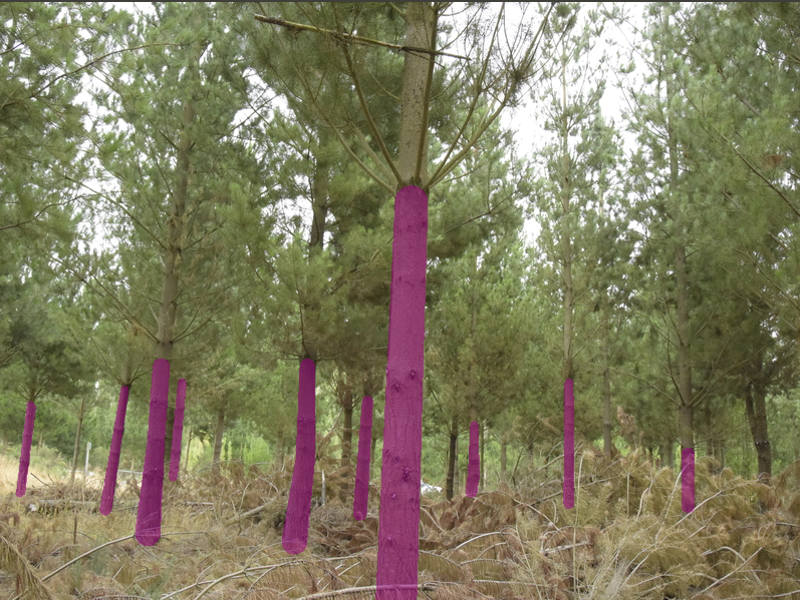
\includegraphics[width=0.9\linewidth]{bootstrap/trees_example.png}

\caption{Example image from the \emph{trees} dataset showing annotated segmentation mask on tree trunks. }
\label{fig:bootstrap_tree}
\end{figure}

\subsection{Related methods}

There are many approximate and interactive machine methods specific to segmentation, in addition to those laid out in Chapter~\ref{chap:introduction}. Each pixel in a mask is highly correlated with its neighbourhood pixels, as such, inputting each pixel is highly redundant; therefore, smart methods can be used to extrapolate segmentation masks from more approximate input. In addition, approximate mask labelling is usually sufficient for most purposes, such as the use of polygons instead of precise boundaries.

An example of active learning specific to segmentation is \cite{Xu2017}, where they focus on finding the nodes (superpixels) which induce the largest change in a \gls{CRF} model.

Semi-supervised machine learning attempts to use existing knowledge or domain properties to infer annotations. For example, using motion cues to give indications of object boundaries \cite{Hong2017}, or using an image classifier to perform object detection by blanking out portions of the image, to determine which parts are important \cite{Bazzani2016}. Semi-supervised methods often substitute for human labour, but in doing so, make sacrifices on the quality and often result in somewhat noisy data. As a result, semi-supervised methods are often used as a means of bootstrapping a model before involving a human annotator, for example as used in \cite{Papadopoulos2016}.


\subsection {Assisted annotation}


\begin{figure}[ht]
\centering
\begin{subfigure}{.5\textwidth}
  \centering
  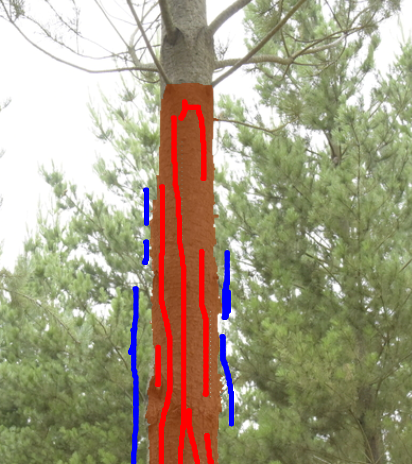
\includegraphics[width=0.9\linewidth]{bootstrap/labelme.png}
  \caption{Labelme mask annotation}  
  \label{fig:bootstrap_labelme}
\end{subfigure}% 
\begin{subfigure}{.5\textwidth}
  \centering
  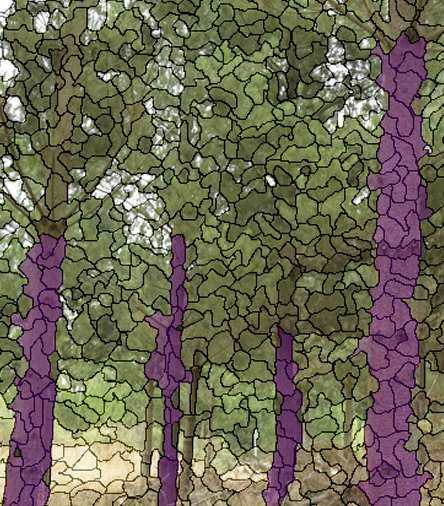
\includegraphics[width=0.9\linewidth]{bootstrap/superpixels.png}
  \caption{Annotation using superpixels}
  \label{fig:bootstrap_superpixels}
\end{subfigure}

\caption{Assisted annotation methods}
\label{fig:bootstrap_annot_method}
\end{figure}


In the initial attempts to annotate a dataset, one of the problems was that using the assisted annotation tools, such as the mask tool in the LabelMe \cite{Russell2007} interface, actually required more work than manually annotating the polygon boundary from scratch. The LabelMe mask tool provides a GrabCut-esque interface where positive and negative stripes can be painted onto an image. Attempts to creating a mask for a tree trunk can be seen in Figure~\ref{fig:bootstrap_labelme}, where annotations are bright red and green. The initially painted stripe provided a rough outline, but many small annotations were needed to make the mask resemble the accurate boundary of the tree trunk.

In \cite{Galloway2017}, the images are segmented using superpixels (clusters of pixels grouped with an unsupervised algorithm), where labelling groups of pixels is substantially less work than labelling individual pixels, and superpixels seem to do well at finding image boundaries where \gls{CNN}s are often imprecise. One difficulty is ambiguity, where multiple classes are covered in one superpixel. In my experience, using superpixels provided imprecise boundaries, and saved little time. An example of the tool with superpixel selection is shown in Figure~\ref{fig:bootstrap_superpixels}.

Deep learning has previously been used to aid in object instance selection. In \cite{Xu2016} a \gls{FCN} is trained to perform semantic segmentation of objects in images as selected by users. Users click on an object (providing positive and negative points), which is provided to the model as distance maps along with the regular colour image data. In \cite{Xu2017} the approach is similar, using a rectangle as an input (also using a distance map), and producing an instance segmentation.


\section{Proposed Method}

The approach is to annotate data and train a model concurrently. First annotate a small number of examples to begin with, to create an initial training set, and use these examples to train an initial model. New examples are then classified by the model, at which point the human annotator fixes any mistakes, and the corrected example is added to the training set. Initially, the annotator will need to fix the majority of the data, and as the model improves such feedback will be required less and less. The idea is that the model will quickly learn the easy cases, which can be quickly ignored to save work, and the annotator will be left to intervene only with the more important challenging cases.

I have used this method to build a small scale tree trunk segmentation dataset, a prototype for use in an automated drone tree pruning project with the aim of pruning lower branches off young \emph{Pinus radiata} tree plantations. This work is intended to allow the drone to see the trees despite the forest. To evaluate methods of dataset construction and evaluate methods of annotation, I wrote an annotation application written with a Qt interface, with tools for drawing on masks and iterating the dataset and refining model proposed annotations.

The work-flow after the first training of some initial  examples was to leave a training process in the background, which would pick up newly created annotations after each training epoch. 

\subsection {Models}

\begin{figure}[h]
  \centering
  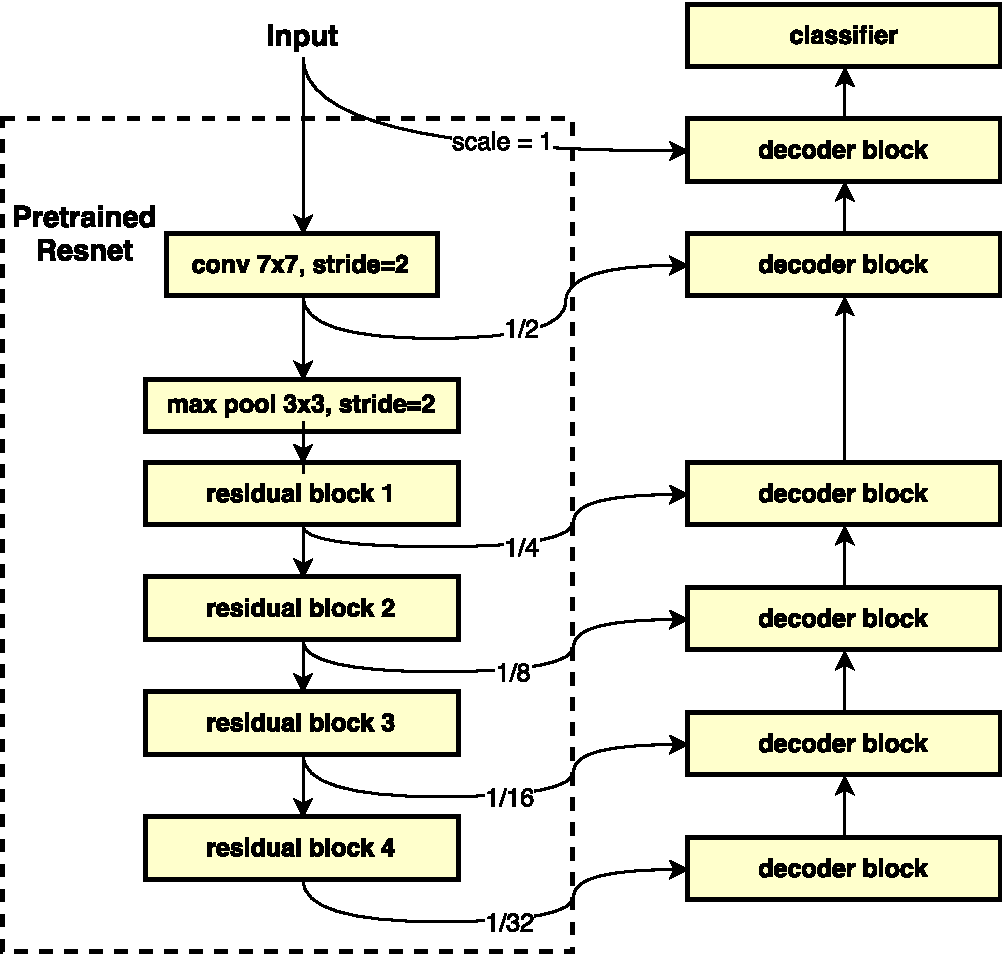
\includegraphics[width=1.0\linewidth]{bootstrap/network.pdf}
  \caption{Encoder--decoder network with pre-trained ResNet as a backbone}  
  \label{fig:bootstrap_network}
\end{figure}
\begin{figure}
  \centering
  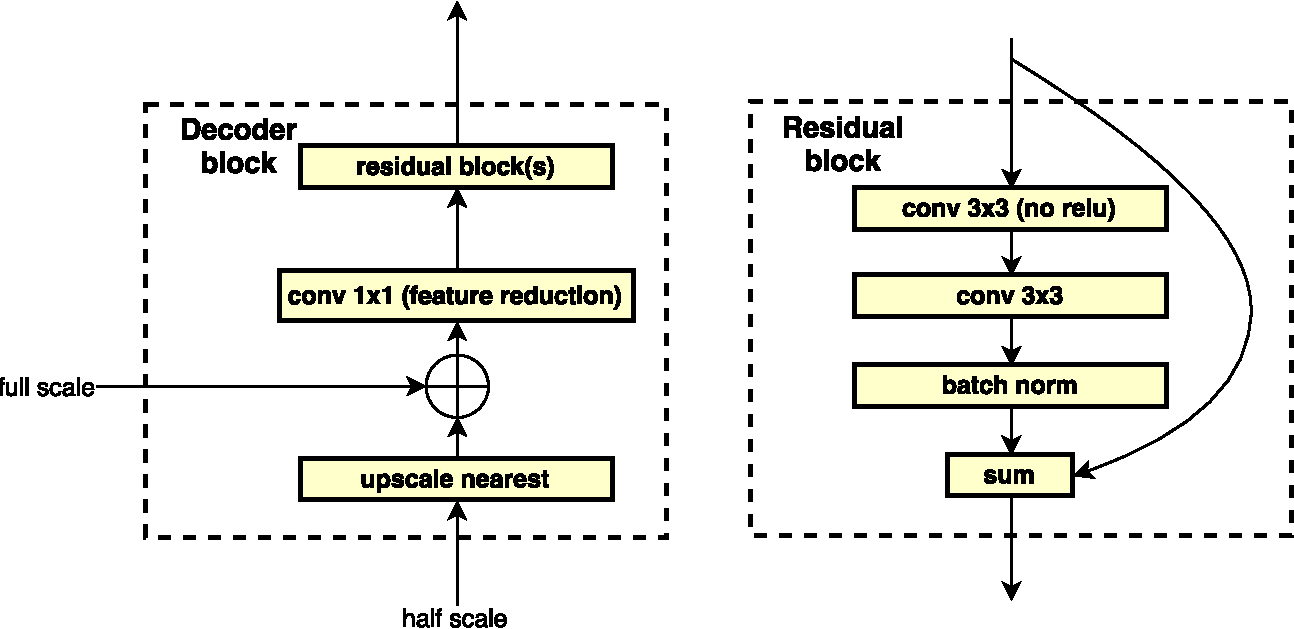
\includegraphics[width=1.0\linewidth]{bootstrap/network_blocks.pdf}
  \caption{Sub-networks. On the left the decoder which combines a low resolution feature map (from a deeper level of the network), with a feature map from the backbone ResNet. On the right the basic residual block with two $3\times3$ convolutions. }  
  \label{fig:bootstrap_decode_block}
\end{figure}

For the image segmentation model, I have used an encoder-decoder with skip connections similar to UNet \cite{Ronneberger2015} (utilising padding and without cropping the skip connections). Each level of the encoder and decoder (at the same resolution) is connected by a skip connection bypassing the lower layers of the network. I focus on two architectures, the first is a pre-trained ResNet model as an encoder with a decoder added, and the second is a symmetrical encoder and decoder. I refer to the first as \emph{pre-trained} and the second as \emph{ladder} in the experiments below.

The architecture based on the pre-trained ResNet \cite{He} is shown in Figure~\ref{fig:bootstrap_network}, with the decoder and residual block used shown in Figure~\ref{fig:bootstrap_decode_block}. The particular ResNet I use is the \emph{ResNet18} from the PyTorch \cite{Paszke2017} model zoo, (the smallest of the various ResNet architectures) with weights trained on the ImageNet dataset. 

The decoder for the pre-trained model uses a single residual block at the point labelled \emph{residual block(s)} in Figure~\ref{fig:bootstrap_decode_block}. The ladder model uses residual blocks of size (1, 2, 3, 3, 3, 3) in both encoder and decoder. The decoder uses $ 1x1 $ convolutions to reduce the feature sizes coming from intermediate layers of the ResNet, the number of features used in the decoder is 16, with 8 additional features at each layer further down. An implicit Batch Normalisation layer and ReLU is present before every convolution.

Of note, the first skip connection is directly the image input, and the second is directly after the $7x7, stride=2$ first convolution used by the ResNet.


\section {Experiments}


\subsection {Loss Function}


I primarily use the \gls{IOU} as a measure of comparison for segmentation. The \gls{IOU} is presented in Equation~\ref{eq:iou} with $ A $ and $ B $ being sets. When training a model, I optimise the Jaccard Distance as a continuous approximation to the \gls{IOU}, this is shown in Equation~\ref{eq:jaccard}.  $ p $ is a binary prediction vector of all output pixels, normalised using the sigmoid function to be between 0 and 1. $ t $ is the binary target vector. Multiplication in these equations is element-wise vector multiplication.


\begin{equation}
IOU = \frac{A \cap B}{A \cup B}
\label{eq:iou}
\end{equation}


\begin{equation}
Jacc = 1 - \frac{p.t}{p.p + t.t - p.t}
\label{eq:jaccard}
\end{equation}



\subsection {Image preparation}

I use images of a fixed size in order to train the network (to process images in batches), however, because the network is a fully convolutional network, inference (and testing) can be performed on images of variable size. I show the effect of this processing later, as compared to training with full-size images with batches of size one.

Data augmentation is used to add variety. I use random scales ($0.8$ to $1.25$), and crops and rotations ($-5$ to $5$ degrees). I adjust colours on a per colour channel basis ($ \gamma = 0.9 $ to $ \gamma=1.1 $ )  $ x_a = x^{\gamma} $.

After scaling and rotation, I then crop an area of the image to $440 \times 440$ pixels (the original image size in the \emph{trees} dataset is $800 \times 600$, down-scaled from the original photos of approximately 25 megapixels).

I employ image whitening as the last step, subtracting an approximate global mean (r, g, b) $ (0.485. 0.456, 0.406) $ and dividing by standard deviation $ (0.229, 0.224, 0.225) $  to ensure consistency with the pre-processing used in ImageNet training with the pre-trained model.



\subsection {Datasets}




I developed a small scale dataset for segmentation of tree trunks in \emph{Pinus radiata} forests (using the approach described). The dataset consisted of 120 images, each containing multiple instances of tree trunks. I labelled the most distinct instances in each image, where some images contained hundreds of background trees. Of the 120 images, I used 30 images for a validation set to use in experimentation in this chapter (which were not used for training).

Along with the \emph{tree} dataset, single classes from the Pascal VOC dataset are used in some experiments. I train with a mix of images from MS COCO \cite{Lin2014} training set along with the Pascal VOC 2012 training set, and use the VOC validation set for validation. The tree images typically contain more instances per image at higher resolution, but significantly fewer images than VOC and COCO images for each category.


\subsection {Minimum viable examples}

\begin{figure}[ht!]

  
\centering
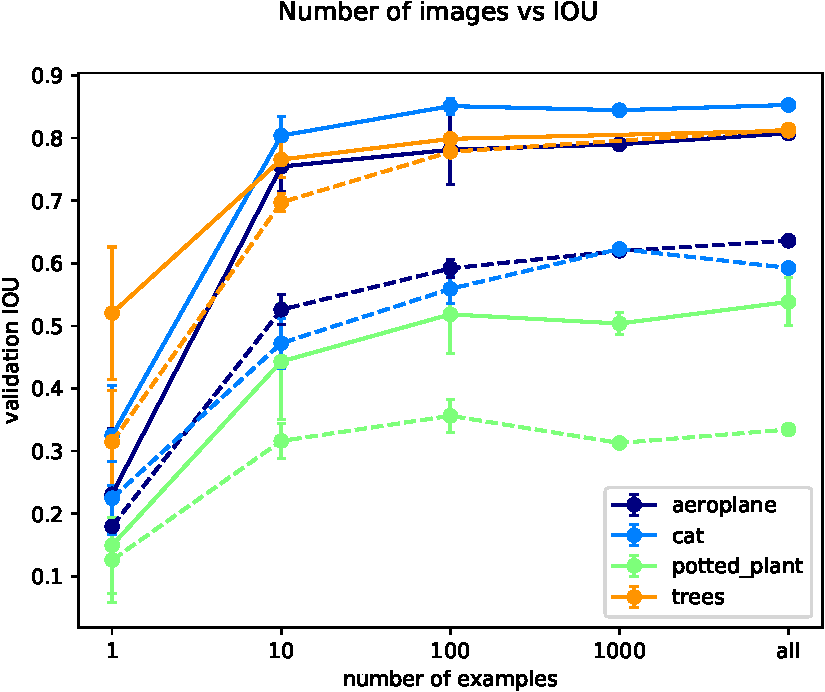
\includegraphics[width=0.9\linewidth]{bootstrap/limit.pdf}
\caption {Validation after training on a limited number of images, solid lines are fine tuned using the pre-trained model, dotted are training from randomly initialisation. }
\label{fig:bootstrap_limited}

\bigskip
\end{figure}

\begin{table}[bht!]
  \centering
 
  \begin{tabular}{ l  l  l}
    examples & training epochs (of 256 images) & repetitions \\
    \toprule
    1       & 8     & 10 \\
    10       & 32     & 4  \\
    100   & 64     & 2 \\
    1000  & 128 & 1 \\
    \bottomrule
  \end{tabular}
  
  \caption{Training parameters for different numbers of examples}
   \label{tab:bootstrap_limit_params}

\end{table}





The effectiveness of involving the model early in the process will be determined by the point where fixing errors in the model's predictions becomes faster than annotating the image from scratch. The effect of the number of examples was studied in \cite{Soekhoe} in the context of transfer learning. One finding was that with smaller numbers of examples, fixing the weights of earlier layers boosted performance when using less training examples.

I performed a simple validation experiment to investigate the effect of using fewer examples. The results can be seen in Figure~\ref{fig:bootstrap_limited}, where in each case the stated IOU is an average over several trials (the number can be seen in Table~\ref{tab:bootstrap_limit_params}), and is additionally averaged over the last three epochs of training. Here I have used classes from the Pascal VOC 2012 for comparison.

It can be seen that even for as few as 10 examples, the validation accuracy is not too different from using a full dataset (1000s of images) in each case, and the difference between using 100 images and the full dataset was minimal in each case. I expected to see the pre-trained model perform much better with a limited number of examples, and this proved to be the case,  it also seems to perform much better in the general case as well. The case matching the initial expectations is the (much more limited) \emph{trees} dataset.



\subsection{Model fine-tuning}

\begin{figure}[!ht]
\centering
  \centering
  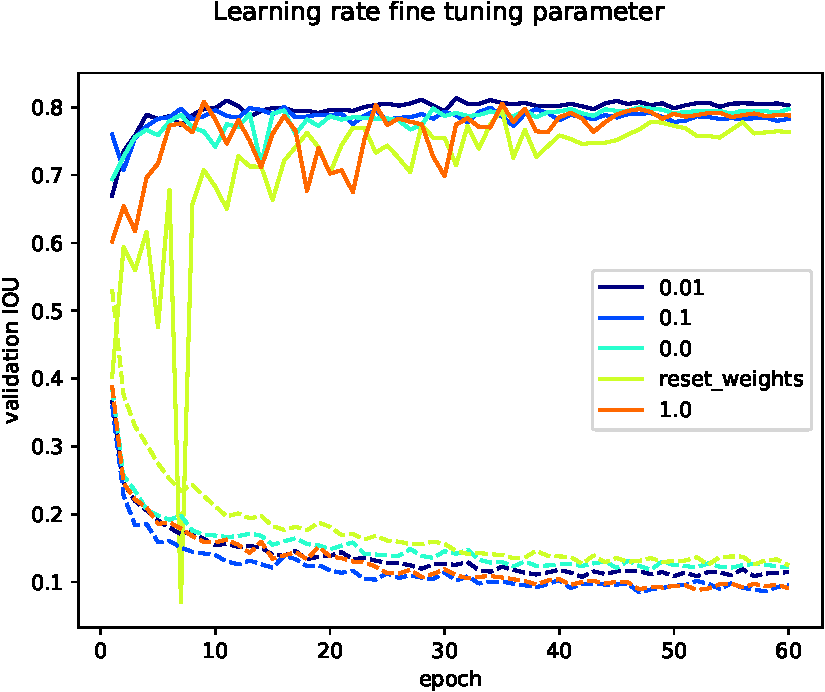
\includegraphics[width=0.9\linewidth]{bootstrap/fine_tuning.pdf}
  \caption{Influence of learning rate modifier for fine-tuning. Solid lines are validation IOU, dotted lines are the mean loss for each training epoch. }  
  \label{fig:bootstrap_fine}
\end{figure}


\begin{figure}[!ht]
  \centering
  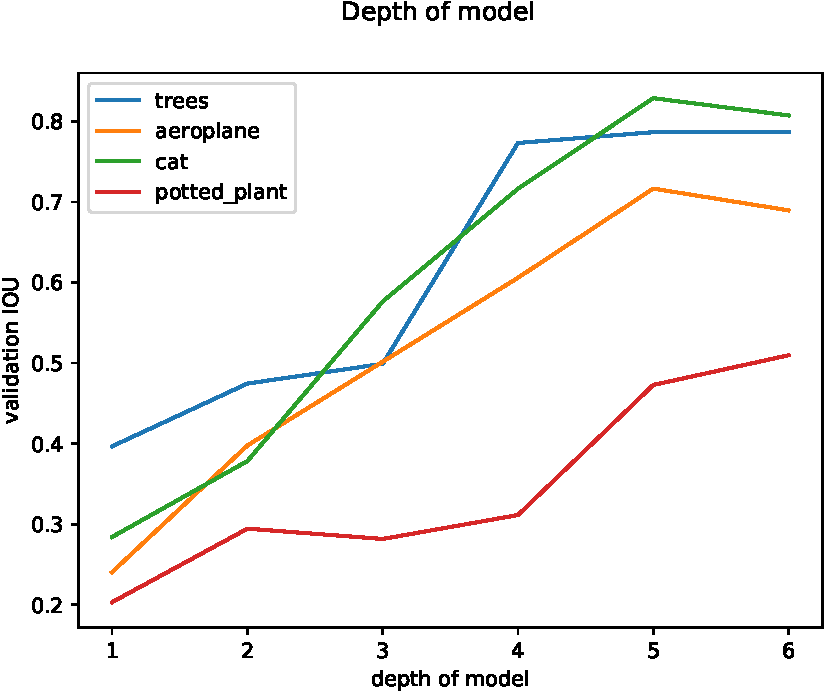
\includegraphics[width=0.9\linewidth]{bootstrap/depth.pdf}
  \caption{Depth of pre-trained model}  
  \label{fig:bootstrap_depth}
\end{figure}


I examined the best parameters for fine-tuning, finding that allowing a small learning rate on the pre-trained model was advantageous. The effects can be seen in Figure~\ref{fig:bootstrap_fine}, where $0.01$ (fraction of the learning rate used for other parts of the model) was advantageous. I used $ 0.1 $ for all other experimentation in this chapter. It can be seen that without the lower learning rate, the pre-trained parameters are disturbed, leading to lower validation accuracy, and without any fine-tuning, the pre-trained parameters are not able to adapt.

Depth of the model is examined, and I experiment with truncating the pre-trained model. Results can be seen in Figure~\ref{fig:bootstrap_depth}, where the depth of the model had a strong positive effect on the output of the model. Given these results, I might consider using a model with even more depth scales. Given the number of convolutions (especially at the lower scales), the ResNet--18 model I have been using has quite a large receptive field, and with more depth scales the receptive field would be larger. In \cite{Peng2017} benefit was found in using very large kernels at the lower levels of the model specifically to enlarge the receptive field.






\subsection {Partial Annotation}


\begin{figure}[!ht]
\centering
\begin{subfigure}[t]{.33\textwidth}
  \centering
  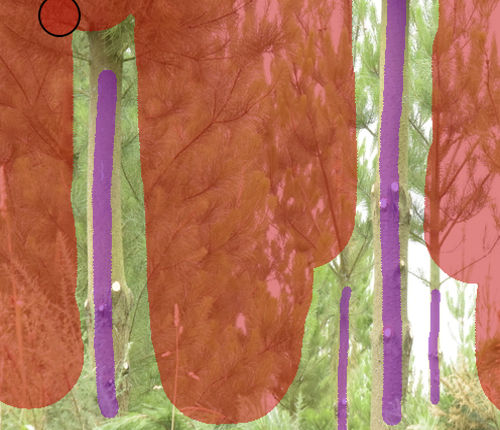
\includegraphics[width=0.9\linewidth]{bootstrap/loose.png}
  \caption{Partial annotation}
  \label{fig:bootstrap_loose_annot}
\end{subfigure}%
\begin{subfigure}[t]{.33\textwidth}
  \centering
  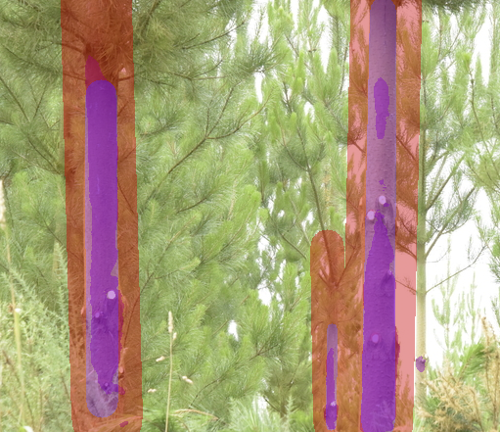
\includegraphics[width=0.9\linewidth]{bootstrap/loose_directed.png}
  \caption{Directed annotation}
  \label{fig:bootstrap_loose_dir}

\end{subfigure}%
\begin{subfigure}[t]{.33\textwidth}
  \centering
  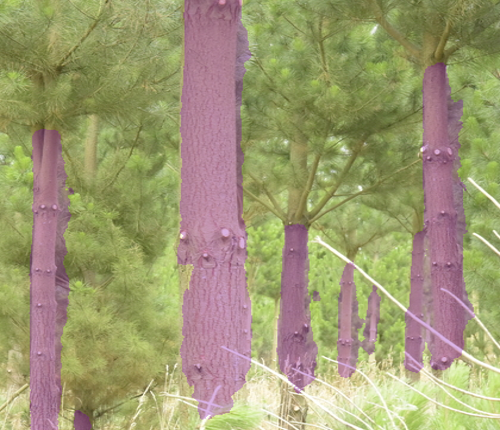
\includegraphics[width=0.9\linewidth]{bootstrap/loose_predictions.png}
  \caption{Partial inference}
  \label{fig:bootstrap_loose_pred}
\end{subfigure}
  \caption{Loose annotation methods in (a) and (b), the red overlay is pixels labelled as background where transparent pixels are unlabelled, (c) shows the  noisy outline produced from partial annotation }


\end{figure}

\begin{figure}
\centering
\begin{subfigure}[t]{.33\textwidth}
  \centering
  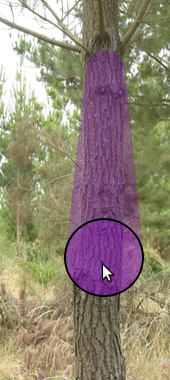
\includegraphics[width=0.6\linewidth]{bootstrap/line_tool.png}
  \caption{Line tool}
\end{subfigure}%
\begin{subfigure}[t]{.33\textwidth}
  \centering
  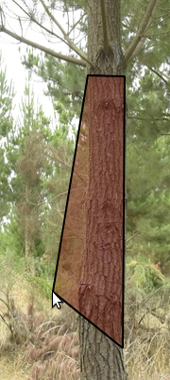
\includegraphics[width=0.6\linewidth]{bootstrap/polygon_tool.png}
  \caption{Polygon tool}
\end{subfigure}%
\begin{subfigure}[t]{.33\textwidth}
  \centering
  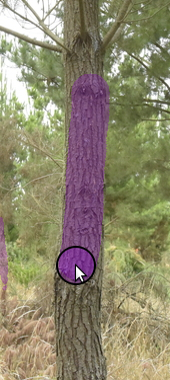
\includegraphics[width=0.6\linewidth]{bootstrap/paint_tool.png}
  \caption{Paint tool}
\end{subfigure}%

  \caption{Label paint tools used in annotation}
  \label{fig:bootstrap_tools}

\end{figure}



An alternative to densely annotating every pixel in an image is to selectively label some pixels while leaving many unlabelled - in the vein of the GrabCut algorithm. I examine this idea for two reasons, firstly annotation of all pixels is finicky or ambiguous (such as the small trees in the background), and secondly to optimise time spent on the annotation of only the most informative pixels (in the vein of active learning).

I firstly looked at partial annotation using paintbrush scribbles on the centre of trees and around the edges of the background. It can be seen that the model trained with partial annotation does not accurately find tree boundaries and has reduced precision as a result, as can be seen in Figure~\ref{fig:bootstrap_loose_pred}. After identifying flaws in that process I compared directed annotation, where I trained a model as I went, in order to guide the annotation process.

For directed annotation, I aimed to densely label the tree instances only where there were mistakes, otherwise leaving the rest of the image not annotated. At the points where mistakes occurred, I made sure to capture the boundaries more accurately. I was again annotating only a small number of easier instances where annotation was clear, unlike in the dense annotation case where many small and ambiguous instances are labelled.

Some statistics can be seen in Table~\ref{tab:loose_exp}, where I can see that both methods of partial annotation are less effective than dense annotation. The second method of directed annotation improves on the precision but reduces recall. It can be seen that the extra supervision of background pixels is indeed useful, and useful supervision is lost by not including it.


\begin{table}[!ht]
  \centering
    \caption{Statistics from re-annotation test set with different levels of approximated annotation, where some pixels are ignored to save annotation time. }
    
  \begin{tabular}{ l  l  l l l l l }
    method & \shortstack{positive \\ pixels}  & \shortstack{background \\ pixels} & \shortstack{ignored \\ pixels} & precision & recall & IoU  \\
    \toprule
    dense annotation    & 10.4\% & 89.6\% & 0\% & 87.8 & 87.3 & 77.8 \\
    loose annotation    & 5.2\% & 67.4\% & 27.4\% & 82.3 & 83.3 & 70.7 \\
    directed annotation & 7.2\% & 54.9\% & 38.0\% & 87.7 & 80.7 & 72.5 \\    
    \bottomrule
  \end{tabular}

\label{tab:loose_exp}
\end{table}

\subsection {Annotation interface experiment}

I performed an exercise in re-annotating the validation set using different tools. The results can be seen in Table~\ref{tab:annotation_exp}, where I used three approaches. The different tools used can be seen above in Figure~\ref{fig:bootstrap_tools}.  The first being a duplication of the initial annotation using the line tool (the tool I initially used to label the dataset), the second being a polygon tool (more commonly used and general purpose than the line tool), and lastly I refined images produced by a trained model, fixing mistakes using the paint tool.

The model I used was a model trained on 30 images (densely labelled) from the loose annotation experiment above. I can see the method of refining model predictions is somewhat faster than the other two input methods, but due to the exercise being undertaken by a single user it is not significantly different ($ p > 0.01 $).

During the annotation, I showed an image of the existing validation image and its annotations side by side to the annotation software, which was necessary to ensure the same task was being performed. The smaller instances in each image were subject to the judgement of the annotator, and other images were extremely crowded or blurry, leading to ambiguity in the annotation process. 

I consider human variability, using a reference annotation created with the same tool operated by the same user. The annotation compared to the reference, only manages a precision and recall of approximately $90\%$. All three input methods were similar in this regard, but display different bias. The polygon tool, for example, was more precise but less complete (lower recall), indicating that the user tended to cut within boundaries defined by the original labelling. 
 
\begin{table*}[!ht]
  \centering
    \caption{Statistics from annotating the set with polygons, lines and then by refining model predictions. Precision, recall and IOU are a comparison with the original validation set. Note figures in brackets are the original statistics of the unmodified predictions from the model}

\noindent\resizebox{\textwidth}{!}{%    
  \begin{tabular}{ l  l  l  l  l  l  l  l }
    method & \shortstack{time \\ per image (s)} & \shortstack{edits \\ per image (s)} & \shortstack{pixels \\ per image} & \shortstack{time \\ per edit (s)} & precision & recall & IoU \\
    \toprule
    polygon    & $79.3 \pm 35.0$  & $12.1 \pm 5.6$ & $52438 \pm 31900$   & $3.9 \pm 1.8$  & $0.94$ & $0.88$   & $0.84$ \\
    line         & $71  \pm 33.4$   & $12.2 \pm 5.6$ & $54781 \pm 33336$   & $2.1 \pm 1.4$ & $0.92$  & $0.90$  & $0.84$ \\
    refine     & $57.3 \pm 40.3$  & $10.8 \pm 6.1$ & $6561 \pm 7102$       & $1.7 \pm 1.4$ & $0.92 (0.89)$   & $0.92 (0.85)$ & $0.85 (0.77)$ \\    
    \bottomrule
  \end{tabular}
}

\label{tab:annotation_exp}
\end{table*}


The confounding feature in the annotation experiment was the need to look backwards and forwards between the two images in order to ensure the correct areas were annotated. In images with many instances, this became a difficult task and identifying small differences between the two became much more difficult. In future, I may perform a more comprehensive user study, by providing an outline of the desired mask for the user to copy directly. This way, the user does not spend any time comparing images and can focus only on the interaction (as a regular user of the annotation tool would).


\subsection{Practical considerations}

Hyperparameters, for example, training rate and model architecture, still need to be determined by validation as soon as enough examples have been obtained to be feasible. I performed some tuning of the hyperparameters (for example the crop size, data augmentation parameters, learning rate) for the purposes of the experiments in this chapter, using the person category of the Pascal \gls{VOC} 2012 dataset; despite the fact that the \emph{tree} dataset is significantly faster to train a similar set of hyperparameters seems to have been suitable.


Practical considerations of having a training process for a \gls{CNN} in the background is that it uses a lot of both \gls{CPU} and \gls{GPU} resources. Running the trainer and the annotation tool together caused significant lag in the annotation tool, which was not otherwise present. It was especially noticeable with a large batch size when the tool would lag in sync with each batch processed. The effect was that annotation became more time-consuming. A simple solution to this would be, for example, to run processes on different machines with a web interface.


\section{Future work}

The interest in tree segmentation was initially for robotic pruning applications and navigation. For this purpose, the segmentation requires further interpretation and fitting. For example, in order to identify tree instances, groups of pixels can be identified then fitted to oriented boxes. This approach does not work for overlapping trees; however, object detection methods also typically struggle with highly overlapping objects.

For these reasons the direction I pursued was to take some of the ideas and lessons learned and apply them to object detection, as can be seen in chapters~\ref {chap:object_detection} and~\ref {chap:annotation}.

For purposes such as identifying foliage of the trees or looking at obstacles in the forest, segmentation does seem like the most natural fit; where one object cannot be easily separated from another. For example, the \emph{Pinus radiata} needles are not distinguishable in the canopy as to which tree they are attached.

\subsection{Segmentation specific}

There is considerable scope for assisted annotation of segmentation datasets, specifically, because the annotation of each pixel is especially laborious. Here are some potential future directions: 

\begin{itemize}
    
\item  {\bf Interactive segmentation} \par
Segmentation often has a class-agnostic element, where the boundary of an object is clear regardless of the object type. User hints can often resolve any ambiguity. An example is interactive object selection \cite{Xu2016, Xu2017}, where user input is combined with image data to segment an object. Large segmentation datasets combined with simulation are used for training, however, an iterative refinement on the specific dataset during annotation may bring further benefit.

\item  {\bf Object selection} \par
Object selection algorithms that can work on the features or outputs from \gls{DNN}s is another idea, such as higher dimensional GrabCut \cite{Xu2016a}, or SuperPixels. Performing Features learned from pre-training on large image datasets is also possible.

\item  {\bf Polygons or shapes} \par
Pixel masks are rarely fully accurate, and drawing tools provide approximate methods for inputting masks in the first place. Directly predicting the kinds of shapes used to input annotations might be a better alternative such as polygons, for example, used in PolygonRNN \cite{Castrejon2017}. Like pixel masks, polygons can be produced by a \gls{NN} and refined by a human annotator. Polygons can be manipulated more easily and better represent the fact that the boundary is an approximation.
\end{itemize}

\section {Summary}

I proposed a bootstrapping method for rapid segmentation dataset creation, involving a feedback loop between human and model. The model trained on partial data was used to assist a human annotator, who then verified the model's predictions and fixed any mistakes. I used this method to create a \emph{tree} dataset for segmentation of \emph{Pinus radiata} trunks (to find trees requiring pruning). I then performed several experiments on this dataset, as well as the Pascal VOC in order to see how I might improve on this bootstrapping method. 

Through several experiments, I determined that fine-tuning a pre-trained model was an effective way to obtain a workable model with very few input images, at least on the \emph{tree} dataset. Partial annotation was explored and found to be less effective than a dense annotation. For this reason, I think that it is more useful to create tools to assist the user to create a dense annotation, rather than making do with more approximate labelling. 
\chapter{Object~Detection}
\label{chap:object_detection} 


\section{Introduction}


\section {Image preparation}

One thing which was noticed in the implementation of the segmentation tool from chapter \ref{chap:bootstrap} was that the original images were often much clearer than the scaled down images for a human annotator to see fine details.

With that in mind I focused on preserving resolution for the annotation process. There may be other reasons to prefer smaller images, such as faster training or inference (which we explore below in section \ref{sec:crop_size}, faster loading, reduced memory size, or reduce disk space. 

The additional benefit to preserving resolution is that performance of a given object detector has generally been shown to be better with higher image resolution, when training on data with a limited number of classes, we hypothesis that it is possible to get away with larger image sizes by using much smaller crops of the original images to train, as long as the objects fit in the image crops. We do some experiments on this idea in \ref{sec:crop_size}.

As a counter example the images in the PASCAL VOC \cite{Everingham2008}, or COCO\cite{Lin2014} datasets have a large range of scales, where many large objects which occupy almost the entirety of the image. For the majority of data experimented on in this thesis, the objects of interest occupy an area much smaller than the whole image size. An analysis of the object sizes in the datasets can be seen in figure \ref{fig:box_sizes}.


\todo{box sizes analysis figure}

\begin{figure}[ht]
\centering
%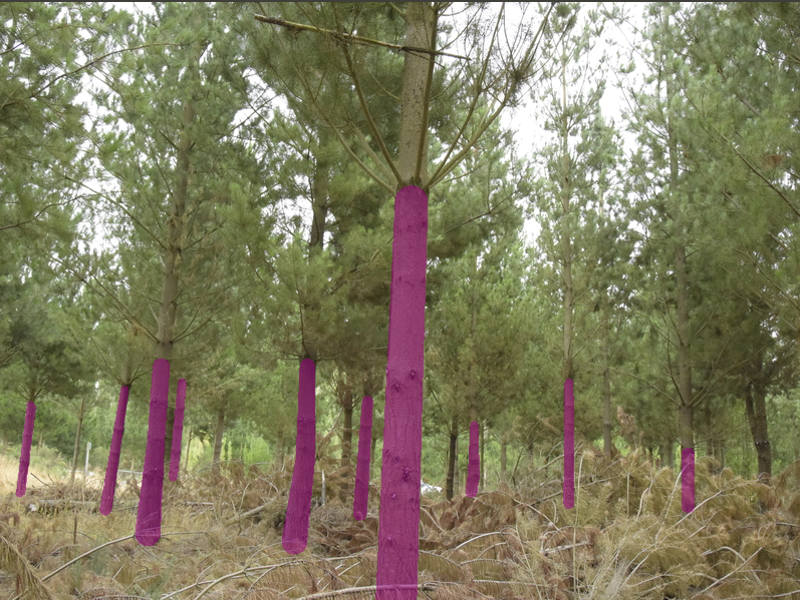
\includegraphics[width=0.9\linewidth]{bootstrap/trees_example.png}

\caption{Object bounding box sizes}
\label{fig:box_sizes}
\end{figure}


Use of simpler, faster models has been successful as the backbone of the object detection network (for example ResNet--18), which enables larger images in both training and evaluation. Time taken for evaluation and training is also much improved relative to using larger networks. For the smaller datasets in our experiments I did not see large improvements in accuracy when using larger backbone networks.

\begin{table}[h]
  \centering
    \caption{Ranges of parameters used for image augmentation, translation occurs as part of a cropping process}
    
  \begin{tabular}{ l  l }
    Parameter & Range \\
    \toprule
    scale (log uniform) & ${3/4}$--${4/3}$  \\ 
    aspect scale  & $ 1 \pm 0.1 $  \\ 

    brightness adjustment (additive) & $ \pm 10 $ \\ 
    contrast (multiplicative) & $ 1 \pm 0.1 $ \\ 

    gamma adjustment & $ \pm 0.1 $ \\ 

    hue shift & $ \pm 5 $ \\ 
    saturation shift & $ \pm 5 $ \\ 
    
    horizontal flips & $ P = 0.5 $ \\ 
    
    \bottomrule
  \end{tabular}
\label{fig:obj_augmentation}
\end{table}

After applying augmentation (photo-metric distortion and scaling) with parameters described in table \ref{fig:obj_augmentation} and image whitening (described below), a region is cropped from the resulting image at random. In the case where the crop region is larger than the input image, an image is created with pixels set to zero and the input image is placed at a random position within the image.

The crop sizes are $600\times600$ unless otherwise specified, for example the tree branch detection uses $300\times300$ due to smaller input images.


We employ image whitening to ensure consistency with ImageNet trained models (used as the backbone of the networks) subtracting mean (r, g, b) $ (0.485. 0.456, 0.406) $ and dividing by standard deviation $ (0.229, 0.224, 0.225) $.


\section {Object detection}

The object detection method I have been using for the following experiments is a modified RetinaNet \cite{Lin2017} as a strong near-state of the art object detector with a simple implementation. RetinaNet is a type of single shot object detector, meaning that it detects all objects together in one pass, as opposed to two stage detectors which first identify sets of bounding box proposals and then have a second pass to refine those box proposals into concrete detections. Single shot detectors (such as \gls{SSD} \cite{Liu2016a} or RetinaNet) typically achieve faster inference and training time by skipping the second refinement phase, at a slight cost of accuracy.  

Many object detection methods are based on sliding windows, where windows of fixed sizes are moved across an image and attempt to match objects of that size at each position. \gls{CNN} based object detectors achieve this using anchor boxes, where the sliding window is replaced by a simultaneous matching of boxes at each point across an image. Using a fixed set of anchor boxes limits the localisation accuracy, so the counter point to matching anchor boxes is also estimating a transformation to refine an anchor box to fit the more specific size of the object.

RetinaNet is based off Feature Pyramid Networks \cite{Lin2017a} which uses feature maps produced at multiple levels of a \gls{CNN} to classify anchor boxes of different sizes, where many smaller anchor boxes match smaller objects on higher resolution feature maps and fewer larger anchor boxes match larger objects. 

The object detection models bear close similarly to the segmentation models discussed and used in chapter \ref{chap:bootstrap}, such as UNet \cite{Ronneberger2015}. \gls{FPN} models utilise shortcut connections in the same way, the major difference from segmentation models is that anchor boxes are predicted at multiple levels, where segmentation models output mask predictions only at one resolution.


\subsection {Network architecture}
\label{sec:architecture}

Some parameters and network architectures differ from the original paper. For the most part the modifications are small things which seem to enable it to learn better on the kind of small datasets used for experiments in this work. 

These include adding extra residual layers to the decoder, shown in figure \ref{fig:detection_network}. It is more similar to the network shown in  \ref{chap:bootstrap} than the \gls{FCN} network. A key difference is that neither the weights between classification sub-networks nor box regression subnets are shared between different scales  (the original shares weights between classification sub-networks). Shared weights were found it to slow down initial training considerably in the initial phase. 

Other differences are necessary to accommodate different box sizes (usually using additional prediction outputs from earlier layers with finer anchor boxes to handle small objects).


\begin{figure}[h]
  \centering
  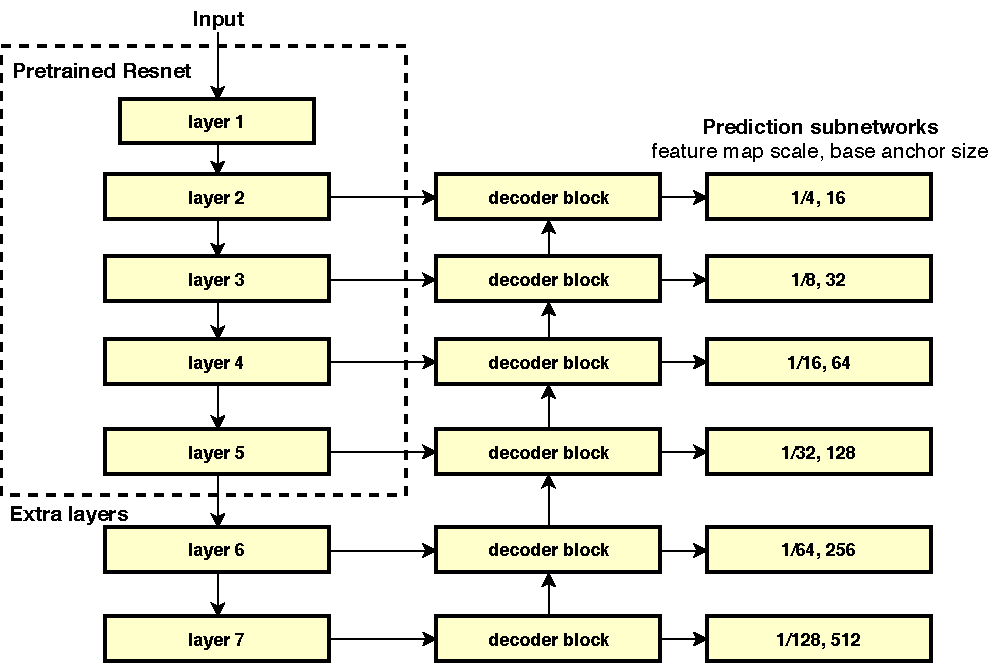
\includegraphics[width=1.0\linewidth]{figures/annotation/detection_network.pdf}
  \caption{Object detection network, built on the backbone ResNet }  
  \label{fig:detection_network}
\end{figure}

% \begin{figure}
%   \centering
%   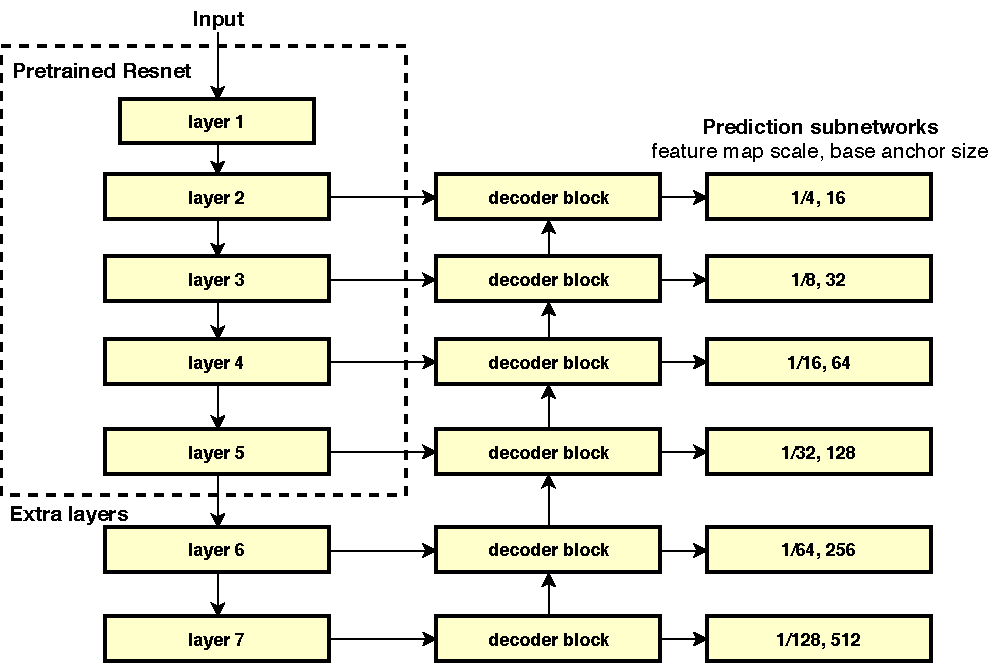
\includegraphics[width=1.0\linewidth]{figures/annotation/detection_network.pdf}
%   \caption{Sub-networks. On the left the decoder which combines a low resolution feature map (from a deeper level of the network), with a feature map from the backbone ResNet. On the right the basic residual block with two $3\times3$ convolutions. }    \label{fig:bootstrap_decode_block}
% \end{figure}

\begin{figure}
  \centering
  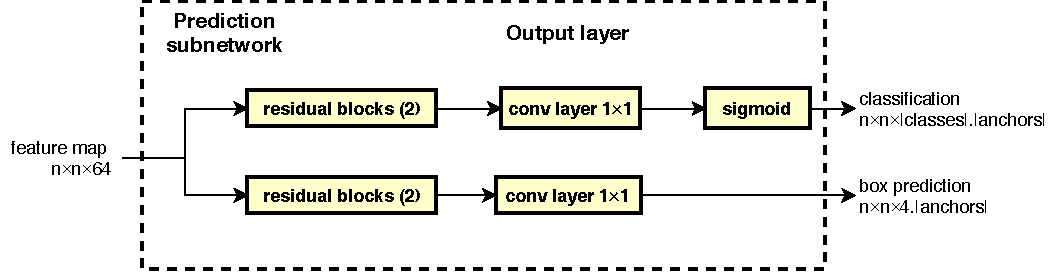
\includegraphics[width=1.0\linewidth]{figures/annotation/prediction_subnet.pdf}
  \caption{Prediction sub-network with two streams, one for classifying anchor boxes with one output per class for each anchor box, the other stream for location regression for each anchor box (shared between classes)}    
  \label{fig:prediction_subnet}  
\end{figure}


\subsection{Anchor boxes}

We use anchor boxes as per \cite{Wang2017}, anchor boxes are the set of default locations and box sizes for which the \gls{CNN} can predict if and which object exists. It is unfeasible to provide a discrete set of boxes large enough to cover all possible object locations, therefore each anchor box is also modified by a scale and translation (details below in section \ref{sec:regression}) to fine tune anchor boxes to fit objects in the image.

Set of anchors boxes are used for each level with aspect ratios $ \in \{0.5, 1, 2\} $ and scales $ \in \{2^0, 2^{1/3}, 2^{2/3}\} $. For each feature map at level $k$, with a base scale of $ 2^{k + 2} $ pixels, the set of 9 anchor boxes (all combinations of aspect and scale) are tiled centred on each feature map pixel. 

In the case of counting, where circles are used for annotation only three anchor boxes are used, only the square aspect ratio is used at the same three scales. For all intents and purposes the circles with radius $r$ are treated as a square box with side lengths $2r$, and the box regression sub-network modified to produce only $3$ outputs (enforcing square aspect ratio for height and width).

Feature maps on levels $3$--$7$ are used for most datasets giving the smallest (square) anchor at $32\times32$ and the largest at $812\times812$ 

For those with smaller objects such as the aerial Adellie penguin counting, the tree branch detection and the seal counting an extra feature map is used giving anchor boxes as small as $16\times16$ and more densely tiled.

In training, anchor boxes are selected by matching on \gls{IOU} overlap with ground truth boxes. Each anchor is matched with the ground truth box with highest overlap. An anchor box matches a ground truth box as a positive if the IOU $ overlap >= 0.5 $, anchors with IOU $ overlap < 0.4 $ are treated as negative, and those boxes with $ 0.5 > overlap >= 0.4 $ are ignored (omitted from either positive or negative for computing loss).

Ground truth boxes will match with potentially many anchor boxes, but those in close proximity and similar size may mean that boxes which would have otherwise matched do not, because anchors cannot be assigned to more than one ground truth.

\subsection {Box regression loss}
\label{sec:regression}


We use the anchor box encoding used in \gls{RCNN} \cite{Wang2017} for the purpose of calculating location loss. The loss is a smooth-L1 loss over four regression targets ($t_x, t_y, t_w, t_h$) giving a transformation from an anchor box ($a_x, a_y, a_w, a_h$)  to a target box from the ground truth ($g_x, g_y, g_w, g_h$). 

The boxes are encoded as the offset of the centre in both directions (in proportion to the box size) and the log scale of height and width. The encoding of the four targets are given as:

\begin{equation}
\begin{split}
t_x = (g_x - a_x) a_w\\
t_y = (g_y - a_y) a_h\\
t_w = log(g_w / a_w)\\
t_h = log(g_h / a_h)\\
\end{split}
\label{eq:encoding_rcnn}
\end{equation}

The localisation loss can be directly computed from these targets and the output of the box prediction sub-network as the sum of the 4 smooth-L1 regressions. Smooth-L1 is a combination of L2 loss near the origin and L1 loss otherwise. It is given as:

\begin{equation}
L_{1;smooth} = 
\begin{cases*}
|x| & if $|x|>\alpha $ \\
\frac{1}{|\alpha|}x^2 & if $|x| \leq \alpha$
\end{cases*}
\label{eq:smooth_l1}
\end{equation}

The commonly used value $\alpha = 0.5$ is used here.

By rearranging the equations we can then do the reverse process and decode bounding boxes from box prediction targets and an anchor box. Here I substitute $ g $ for $ p $ to denote a bounding box prediction instead of a ground truth.

\begin{equation}
\begin{split}
p_x = a_x + t_x  a_w\\
p_y = a_y + t_y  a_h\\
p_w = exp(t_w) a_w \\
p_h = exp(t_h) a_h\\
\end{split}
\label{eq:decoding_rcnn}
\end{equation}

\subsection {Classification loss}
\label{sec:loss}

The experiments use a modified version of the Focal Loss \cite{Lin2017} to handle the class imbalance (negative vs. positive) present when sampling anchor box predictions densely.

Focal Loss \cite{Lin2017} re-weights the standard \gls{BCE} loss function to deal with a large number of easy negative examples in object detection. This enabled dense sampling of negative examples present in an image. The standard approach in to dealing with the imbalance between positive and negative examples has been to sample the most significant negative examples to provide a certain positive to negative ratio.


As defined \cite{Lin2017}, we use the same terminology and variable naming for consistency. The basic two class \gls{CE} equation for binary prediction from the model classifier $p \in \left[0, 1\right]$, and label $y \in \{0, 1\}$  is given:

\begin{equation}
CE(p, y) = 
  \begin{cases*}
  -log(p) & if $y = 1$\\
  -log(1-p) & otherwise\\
  \end{cases*}
\label{eq:cross_entropy}
\end{equation}


The cross entropy can be rewritten by defining $p_t$ the prediction relative to the given label.

\begin{equation}
p_t = 
  \begin{cases*}
  p & if $y = 1$\\
  1 - p & otherwise\\
  \end{cases*}
\label{eq:class_prob}
\end{equation}

Allowing the \gls{CE} equation to be rewritten more simply:

\begin{equation}
CE(p_t) = -log(p_t)
\label{eq:short_cross_entropy}
\end{equation}


In order to deal with class imbalance the key idea of \cite{Lin2017} was to re-weight the classification loss to be smaller for well classified boxes (small $p_t$) and to be relatively much larger for badly classified boxes (large $p_t$). This was achieved by multiplying the cross entropy by a factor of $(1 - p_t)^\gamma $ with parameter $\gamma$ a sharpening parameter, to give the focal loss:

\begin{equation}
FL(p_t) = - (1 - p_t)^\gamma log(p_t)
\label{eq:focal_loss_p}
\end{equation}

Another way of dealing with class imbalance is to weight one of the classes (in the binary case given here either the positive c

A balanced cross entropy loss can then be written by adding a class weighting $\alpha \in \left[0, 1\right]$ the weight for the positive case in the two class setting, and an analogous $\alpha_t$:

\begin{equation}
\alpha_t = 
  \begin{cases*}
  \alpha & if $y = 1$\\
  1 - \alpha & otherwise\\
  \end{cases*}
\label{eq:balanced_weight}
\end{equation}

Then the balanced, focused, cross entropy is defined:

\begin{equation}
FL(p_t) = -\alpha_t (1 - p_t)^\gamma log(p_t)
\label{eq:focal_loss}
\end{equation}


I adopt the parameters given in \cite{Lin2017}, using $ \gamma = 2 $, and $ \alpha = 0.25 $.

\subsection{Inference and Non-maxima suppression}

In training a large set of anchor boxes are trained to classify each object detection (those overlapping each anchor box by $0.5$ or more). For the purposes of inference detecting more than one box for each object is undesirable, so a greedy non maxima suppression is used to eliminate multiple detections of the same object.

In this work a standard \gls{NMS} procedure as per \cite{Wang2017} is used, where boxes are selected from most confident to least confident, boxes overlapping the selected box (of lower confidence) are eliminated.


\section {Learning schedule and averaging}
\label{sec:schedule}

In order to facilitate continuous learning where examples are added over the training lifetime, a cyclical learning rate is used and relatively short learning epochs are used. Epochs are set at a fixed size ($1024$ unless otherwise specified), using randomised sampling. Learning rates are set for each batch, reducing over an epoch by a factor of $10$, using a logarithmic interpolation shown in equation \ref{eq:lr}. Where $base$ is the base learning rate, and $t$ is varied from $0$ to $1$ across the epoch.

\begin{equation}
lr(t) = exp(ln (base) * (1 - t) + ln(base/10)  * t)
\label{eq:lr}
\end{equation}


% \subsection {Single vs. multi class}
% \label{sec:multi_class}


\section {Experiments}
\label{sec:experiments}

\subsection {Crop size}
\label{sec:crop_size}


\subsection {Effect of scale}
\label{sec:detection_architecture}



\subsection {Incremental classes}
\label{sec:incremental}



\chapter{Image~Annotation}
\label{chap:annotation} 

This chapter describes the design, implementation of a human in the loop object detection system and details it's use annotating real datasets.

\section{Introduction}

\section {User interface}

The user interface of the system resembles a diagram editor, where shapes (boxes, circles, polygons) can be drawn over an image and manipulated in the usual ways. Shapes can be moved by selecting and dragging, resized by scrolling the mouse wheel or by moving control points. 


\subsection {Auto annotation}

At the core of the user interface is providing immediate feedback on images viewed by the user.


\subsection{Active learning}


\subsection {Confidence thresholding}

Choosing the confidence threshold is an important parameter for inference using an object detector. The consequence of an incorrect detection threshold is extra work for the annotator, either having to delete too many false positives or be left with too many boxes to draw. Many times, especially with difficult image detection problems an weak detector will produce many detections (some true positives, some false positives). The weak detector will not be able to separate these detections by confidence value. Using human verification there exist some obvious strategies to separate the true positives from the false positives, while still not missing too many objects altogether. 

\begin{itemize}
    \item Set a low detection threshold and have the user delete false positives
    \item Set a low detection threshold and have the user select true positives
    \item Set a high detection threshold and have the user draw boxes around missed detections
\end{itemize}

Each of these strategies has a valid place. If detections are so noisy and if the location predictions are very noisy (for example when the detector is very weak, such as near the start of the process) - having the user draw boxes is often the only option. Some of these strategies are amongst used by \cite{Konyushkova2017} which attempts to solve this problem differently, by attempting to automatically determine the best interface for a given image.

Deleting false positives is often the best option if true positives outnumber the false positives, or if the false positives are easy to select (if they're grouped together, for example). Selecting true positives is often the best option if the false positives outnumber the true positives. 
There exists another strategy which has the best of both worlds. Two thresholds can be used, a high confidence threshold can be used for eliminating false positives (such that when using this threshold the number of false positives is low). Detections between the high and low confidence thresholds can be considered for selection as true positives (such that the number of true positives requiring selection is low).


\begin{figure*}[h]
\centering
\begin{subfigure}[t]{0.5\linewidth}
  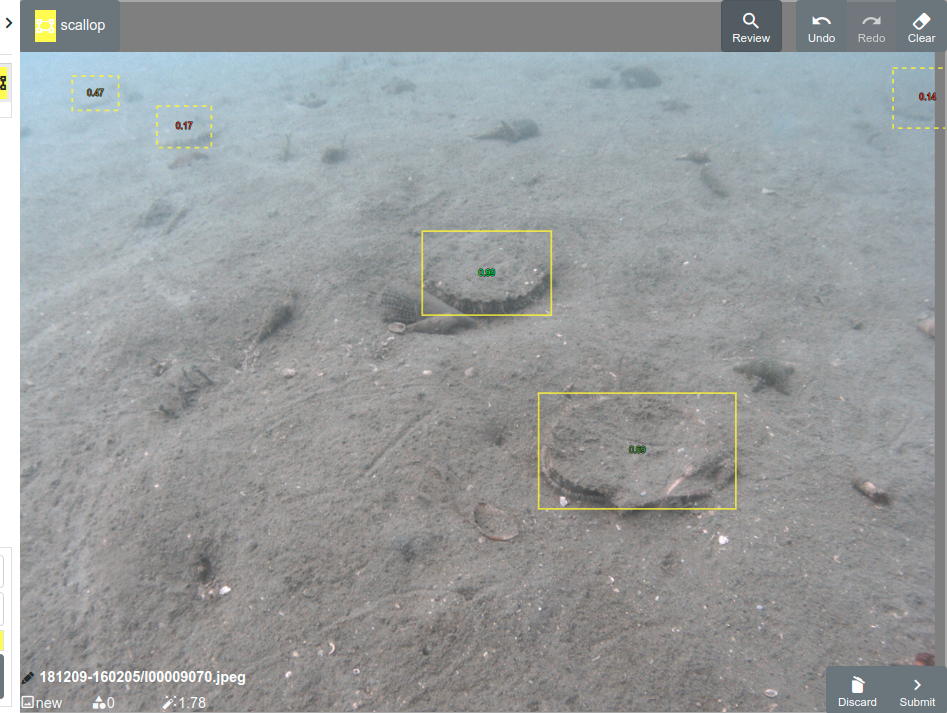
\includegraphics[width=1.0\linewidth]{figures/annotation/scallop/review_mode.png}
  \caption{}
\end{subfigure}%
\begin{subfigure}[t]{0.5\linewidth}
  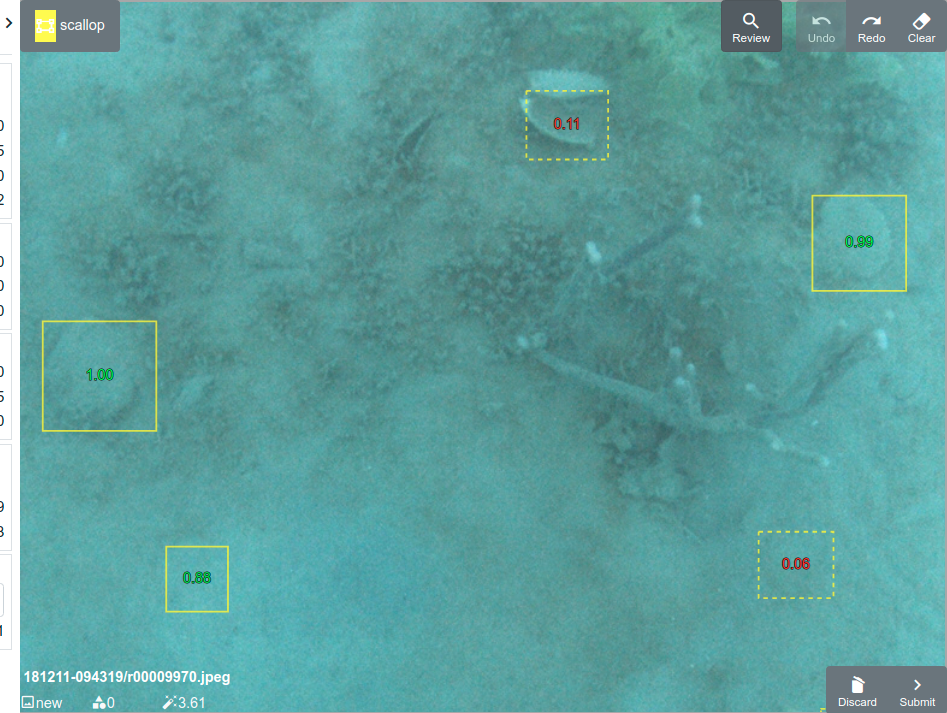
\includegraphics[width=1.0\linewidth]{figures/annotation/scallop/false_positive.png}
  \caption{}
\end{subfigure}%
\caption{Review mode used on two fresh images from the scallop dataset, (a) showing an ideal case (b) showing an image with a high confidence false positive among low confidence detections}
\label {fig:confidence}
\end{figure*}



I provide a key which toggles between showing the detections in the mid range between the two thresholds, when the key is held a click is used to confirm a detection as a true positive. I term this toggle ``review mode''.  An example showing the mechanic of this can be seen in figure \ref{fig:scallop_review}. In one image the ideal situation is shown where three scallops are detected in the background (with low confidence), where otherwise they might have been ignored. In the other, a less useful case where the low confidence detections are false positives, and one of the high confidence detections is also a false positive, despite this the user saves time by ignoring the other low confidence detections.

The other advantage of this strategy are that it can bring the annotators attention to areas of the image which may have gone unnoticed. I have noticed in particular with the underwater scallop images that the detector usually did a good job at bringing attention to the more uncertain scallop instances. It also provides useful feedback to the annotator of the progress of the current object detector. 




\begin{figure}[h]
\centering
% \begin{subfigure}[b]
% %   \includegraphics[width=1.0\linewidth]{figures/annotation/confidence_training.pdf}
%   \caption{}
% \end{subfigure}

% \begin{subfigure}[b]
% %   \includegraphics[width=1.0\linewidth]{figures/annotation/confidence_validation.pdf}
%   \caption{}
% \end{subfigure}

\caption{ The evolution of confidence levels as training progresses, in (a) training and in (b) validation }
\label {fig:confidence}
\end{figure}

During training it can be seen that the confidence levels provided by the object detector vary with regard to training time. This can be seen in figure \ref{fig:confidence}, comparing the distribution of confidences between training and validation. This is a known property of neural network classifiers \cite{Guo2017}.

In future I would like to investigate calibration of thresholds using validation. This can be done by continually adjusting thresholds to match a certain ratio of false positives to false negatives (the desired ratio to be set by the user), alternatively prediction confidence itself can be calibrated to attempt to provide more consistent values. Confidence scores can be calibrated by scaling scaling outputs prior to applying softmax normalisation \cite{Guo2017}. For the purpose of object counting I use the former method to select thresholds. In order to provide the most unbiased estimate of counts the confidence is selected to give an equal ratio of false positives to negatives.


\subsection {Reviewing and verifying}

In crowd sourcing image annotation software, verification is required to ensure the consistency of the annotations. Verification prevents malicious or incompetent users to spoil the data and provides some assurance that the end result is of high quality. 



Reviewing a previously edited image and it's annotations is presented to the user in a very similar way to viewing a newly opened image. The main differences lie in how the global threshold affects the displayed annotations. 





\begin{figure}[h]
  \centering
  \includegraphics[width=1.0\linewidth]{figures/annotation/penguin_refine.pdf}
  \caption{Illustration of a human annotator refining a set of bounding box predictions }  
  \label{fig:penguin_refinement}
\end{figure}




\section {Implementation}

\subsection{Server and client}

\begin{figure}[h!]
  \centering
  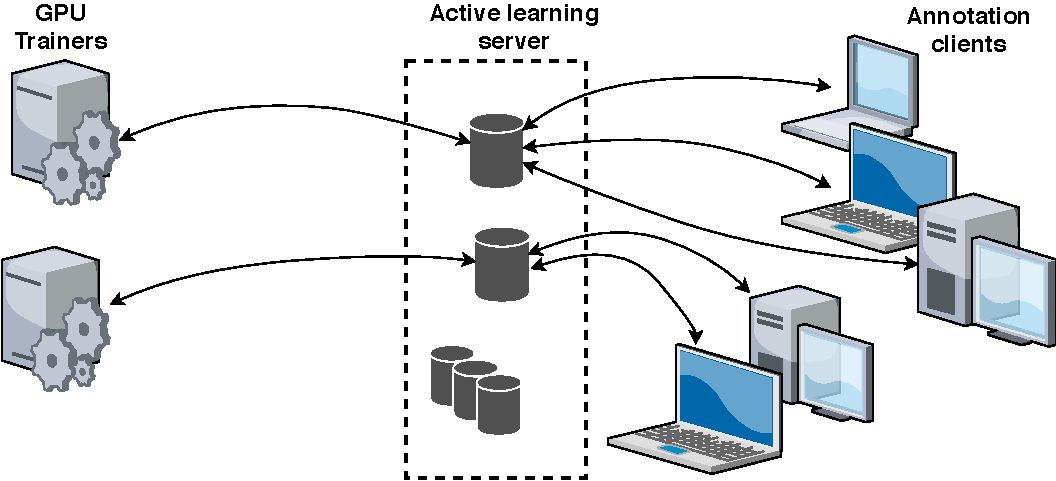
\includegraphics[width=1.0\linewidth]{annotation/connectivity.pdf}
  \caption{Connectivity of the annotation system}  
  \label{fig:connectivity}
\end{figure}

The system can be broken down into three parts running separately but communicating. This can be seen in figure \ref{fig:connectivity}. There exists a server process which sits in the middle and acts as a conduit for communication, a store of data and a serialisation of state. The server sits in the middle and communicates with both trainers and clients.

The main reason for splitting server and trainer was initially for practical reasons, the client and server both written in \gls{GHC} Haskell, and deep learning frameworks written mainly in python. The server and client are written in Haskell, the former running naively, the later compiled to JavaScript using \gls{GHCJS}. 

Splitting server and trainer does also provide some advantages. It allows the server to act as a portal through which users can work on several datasets. One or many trainers can be shared concurrently or time shared without having to run new instances of the server. 

The current reality is more simple, a single trainer services the server and operates on a first come first served basis. One dataset at a time is trained, until a period of inactivity (no images submitted for $ n $ training epochs). A trainer still services clients working on inactive datasets by providing detection (best models for each dataset are kept in \gls{CPU} memory), but trains on only one dataset at a time. 

\begin{figure}[h!]
  \centering
  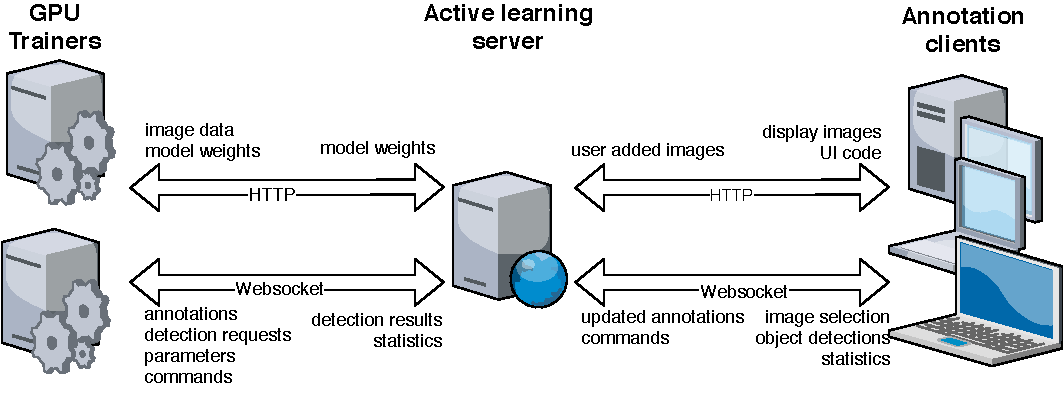
\includegraphics[width=1.0\linewidth]{annotation/data_flow.pdf}
  \caption{Data flow between services for the annotation system}  
  \label{fig:data_flow}
\end{figure}

An illustration of the data flow which occurs between different parties can be seen in figure \ref{fig:data_flow}. Large binary data is shared using \gls{HTTP}, for example model weights and images are distributed this way. Other data is communicated over websocket connections using \gls{JSON} text. Examples of this includes synchronising new annotations, and image statistics, which are continually updated to the client for the purpose of the example selection in active learning.

Image data is stored on the server and transmitted as required to trainer and client. Images are sent to client for viewing and inspection, and to the trainer for training and cached for more efficient loading. 

Models are stored on the server and requested by the trainer as required, for example when starting training on a dataset the trainer requests the previously stored model weights. The trainer also caches copies of weights (as required) of recently used models for the purposes of inference as required by the client for every image opened. Given the large size of data involved in transmitting large images, and also updating model weights, the trainer is suited to exist on the same local network as the server. 



\subsection {User interface}

I provide a web interface for the following reasons:

\begin{enumerate}
    \item No installation
\end{enumerate}
Any system with a web browser will be fine, software utilising complex computer vision and GPU programming libraries is often hard to package for easy installation. A web interface sidesteps these difficulties.
\begin{enumerate}[resume]
    \item Local GPU not required
\end{enumerate}
By running the trainer on another system anyone can use the system without requiring a local GPU. One of the problems with usability from my earlier work was that GPU intensive tasks running on the same computer ruin the responsiveness of a user interface. To my knowledge there is no good way to run a heavy \gls{GPU} intensive processing task at a low priority such that the user interface remains responsive.
\begin{enumerate}[resume]
    \item Enables collaborative annotation/crowd sourcing
\end{enumerate}
A web interface enables a straightforward extension to use for larger scale annotation with multiple users annotating the same dataset. An example can be seen in \label{fig:connectivity} showing two groups of users operating on the same datasets.


The trade-off for a web interface is in performance, it prevents doing computationally heavy calculation in the client, especially for loading and processing large images. For this work we face no such difficulty, though for example a super pixel based tool for mask annotation would be more challenging. With newer web technologies such as WebAssembly \cite{Haas2017} to run code at near native speeds in a browser, and WebGL shaders for GPU programming.











\section{Annotation studies}

\subsection {Penguins}
\subsection{Tree branch intersections}
\subsection{Scallop}


\section{Counting}

\subsection{Adelie Penguins}
\subsection{Waddell Seals}




\section {Reviewing mistakes}


\bibliographystyle{unsrt}
\bibliography{references}
\end{document}